\chapter{Results} \label{results}
As mentioned in the previous chapters, compared with the upsampling approaches in other papers, this thesis has many updates in the model, data processing and loss function, so this chapter will mainly focus on the evaluation of these three aspects, but also some others. Since only its amplitude is useful in the visualization of range-Doppler map, the evaluation loss will be only based on the amplitude and only in the frequency domain as mentioned in chapter \ref{loss functions}. Furthermore, during the training process, the input of the model may be processed in many different ways, and the pipeline uses the processed output to calculate the training loss, whereas in the evaluation phase, the data will be converted back to the complex value without logarithm and normalization to calculate the evaluation loss.

Since there are too many combinations, in order to make an intuitive and clear comparison, each evaluation will ensure that other parameters are the same, and only one difference will be compared each time, and the most suitable one will be determined for the subsequent evaluations. Due to the large number of evaluation cases, the size of the model and data are selected as a small one, whereas a large model will be trained with the whole dataset at the end. The evaluation indicators are mainly divided into two parts, one is the values of the evaluation losses. The smaller the evaluation loss, the better the model. The other is the visual effect of the generated super-resolution range-Doppler map.

\section{Models comparison} \label{models comparisons}

Firstly, a model shall be determined to evaluate various subsequent processing methods and loss functions. Here, the classical loss function and common processing methods are used, namely the \gls{mse} loss function for training, convolutional layer as the dimension processing layer for the prime range shape and transposed convolutional layer as the upsampling layer, using the real and imaginary representation type, and without any logarithm or normalization operations, that is, the \gls{mse} loss function is calculated in linear scale.

\begin{table}
    \centering
    \caption{Evaluation losses of different models in the case of the MSE and common processing methods.}
    \label{models comparison in the case of the MSE and original processing methods}
    \begin{tabular}{l|c|c|c|c|c|c}
        \hline
        Models comparison & \#Params & MSE & SDR & LSD & WMSE & Perceptual \\
        \hline
        Interpolation & 0 & 3.570 & -3.620 & 0.750 & 0.774 & 28.010 \\
        \hline
        CNN\_simple & 103,684 & 2.164 & -5.028 & \textbf{0.441} & 3.599 & 25.133 \\
        \hline
        UNet\_simple & 93,162 & 1.352 & -2.872 & 0.600 & 1.034 & 22.014 \\
        \hline
        UNet\_concat & 96,746 & \textbf{1.275} & -3.609 & 0.552 & 0.968 & \textbf{21.847} \\
        \hline
        DP & 113,964 & 3.212 & -4.926 & 0.611 & \textbf{0.163} & 23.583 \\
        \hline
        SwinIR+DP & 97,252 & 1.754 & \textbf{-5.787} & 0.503 & 0.314 & 22.764 \\
        \hline
        SwinIR+Swin & 111,624 & 1.541 & -4.505 & 0.546 & 1.104 & 26.381 \\
        \hline
    \end{tabular}
\end{table}

\begin{figure}
    \centering
    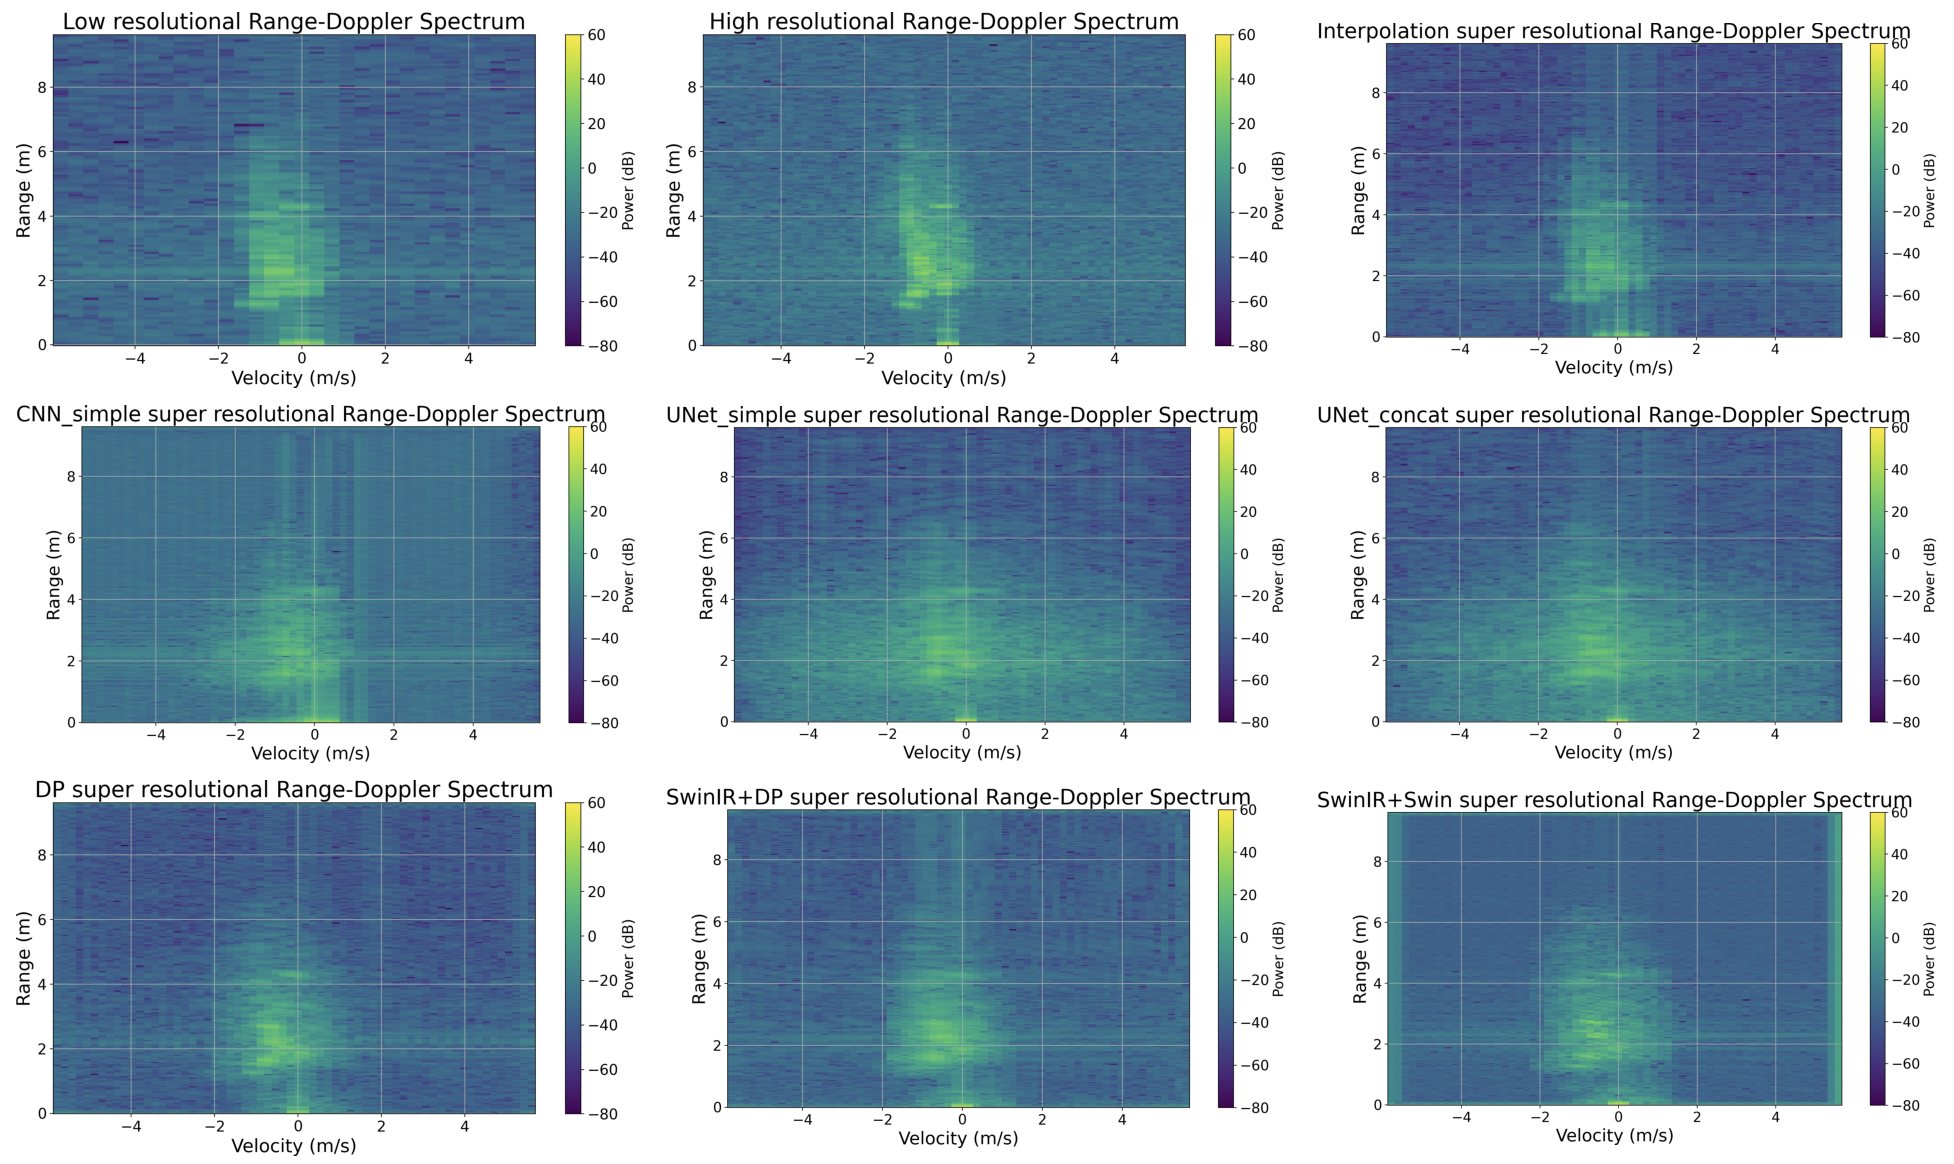
\includegraphics[scale=.45]{thesis/figures/evaluation_models_1.png}
    \caption{Super-resolution range-Doppler maps of different models in the case of the MSE and common processing methods.}
    \label{evaluation models 1}
\end{figure}

From the results of the evaluation losses in Table \ref{models comparison in the case of the MSE and original processing methods}, most models have one good result, but from the perspective of super-resolution range-Doppler maps shown in Figure \ref{evaluation models 1}, the basic \gls{cnn} model and both UNet models are not as good as the Transformer models, since there seems to be some information loss in the area of the strong signals. Among them, the \gls{dp}-\gls{tf} Transformer model and \gls{swinir} architecture with \gls{dp} Transformer block model seem to be better at present. The subsequent evaluations on the processing methods and training loss functions will temporarily use the \gls{dp}-\gls{tf} Transformer model.

According to the optimal processing methods evaluated in section \ref{processing methods comparisons} and the loss combination evaluated in section \ref{training loss functions evaluations}, we evaluate again the models. Table \ref{models comparison in the case of the LSD and new processing methods} and Figure \ref{evaluation models 2} show the evaluation losses and super-resolution range-Doppler maps in the new case.

\begin{table}
    \centering
    \caption{Evaluation losses of different models in the case of the loss combination and new processing methods.}
    \label{models comparison in the case of the LSD and new processing methods}
    \begin{tabular}{l|c|c|c|c|c}
        \hline
        Models comparison & MSE & SDR & LSD & WMSE & Perceptual \\
        \hline
        Interpolation & 2.485 & -6.825 & 0.435 & 1.305 & 21.898 \\
        \hline
        CNN\_simple & 3.574 & -7.722 & 0.345 & 0.227 & 26.649 \\
        \hline
        UNet\_simple & 3.126 & -7.918 & 0.338 & 0.225 & 19.148 \\
        \hline
        UNet\_concat & 1.992 & \textbf{-8.355} & \textbf{0.320} & 0.175 & 17.916 \\
        \hline
        DP & 1.731 & -5.375 & 0.380 & 0.179 & \textbf{12.320 }\\
        \hline
        % DP & 2.052 & -5.530 & 0.377 & 0.192 & 11.997 \\
        % \hline
        SwinIR+DP & 1.662 & -6.415 & 0.360 & \textbf{0.128} & 16.903 \\
        \hline
        SwinIR+Swin & \textbf{1.619} & -6.392 & 0.360 & 0.134 & 15.662 \\
        \hline
    \end{tabular}
\end{table}

\begin{figure}
    \centering
    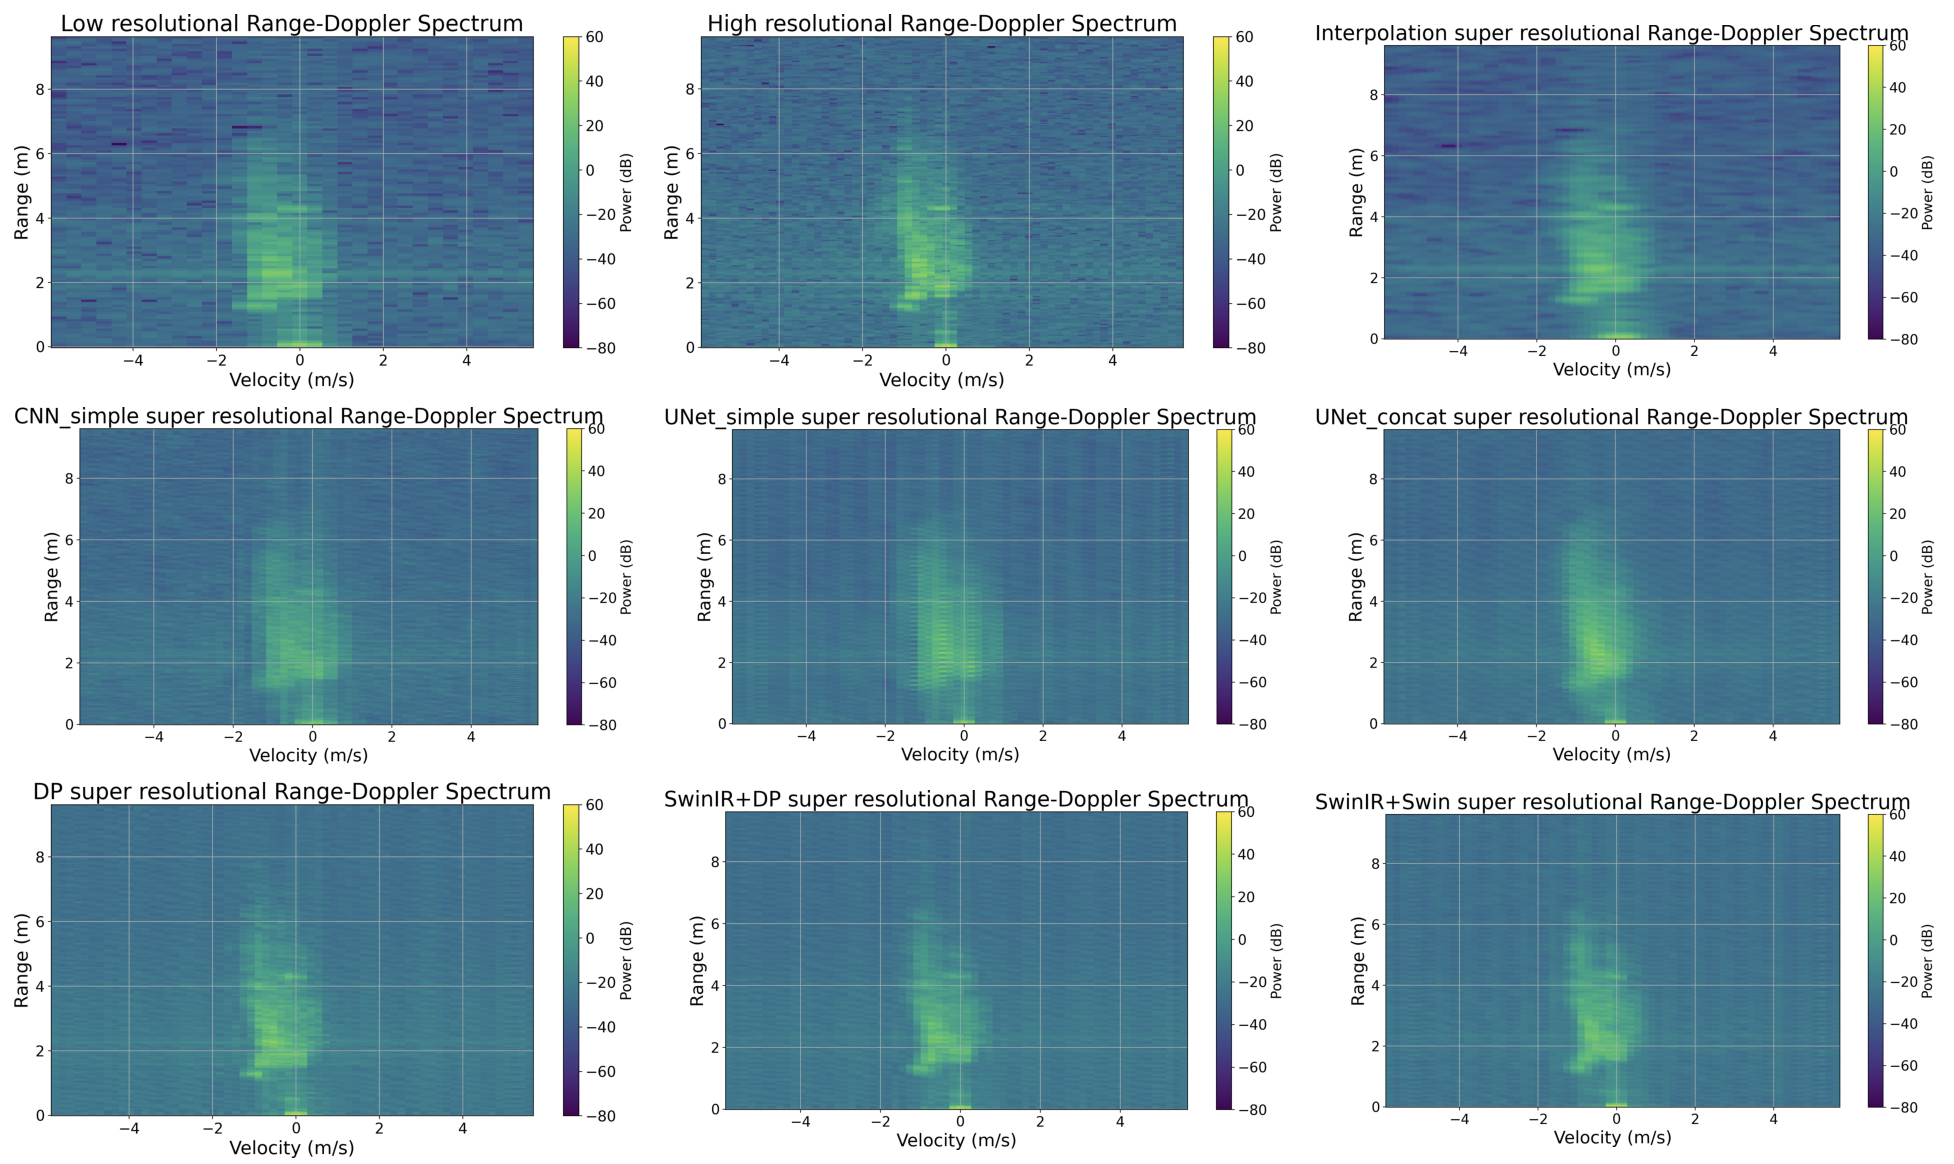
\includegraphics[scale=.45]{thesis/figures/evaluation_models_2.png}
    \caption{Super resolution range-Doppler maps of different models in the case of the loss combination and the new processing methods.}
    \label{evaluation models 2}
\end{figure}

After using the new combination of the processing methods and the loss combination, most of the evaluation losses are optimized. Furthermore, visual effect of the super-resolution range-Doppler map is improved as well. Some peaks in the high-resolution range-Doppler map can be clearly seen in the super-resolution range-Doppler map, especially in the Transformer models. Balanced by the evaluation losses and the visual effect, the \gls{dp}-\gls{tf} Transformer model and \gls{swinir}+\gls{dp} model are still better, where \gls{dp}-\gls{tf} Transformer model performs well in the perceptual loss while \gls{swinir}+\gls{dp} model is good at the other losses. Since the peaks look clearer in \gls{dp}-\gls{tf} Transformer model, following sections will keep using \gls{dp}-\gls{tf} Transformer model.


\section{Processing methods} \label{processing methods comparisons}
Based on the above \gls{dp}-\gls{tf} Transformer model, this section will compare the different combinations of the processing methods, namely input data representation, dimension processing types, upsampling types, logarithm and normalization operations.

\begin{spacing}{1.5}
\textbf{\large{Input data representation}}
\end{spacing}
While processing complex-valued data, there are three types of the input data representation, namely real and imaginary, amplitude as well as amplitude and phase. The other processing methods keep no dimension processing layer, the transposed convolutional upsampling layer, and do not use any logarithm and normalization operations, which means only the representation type is changed compared with the first case in section \ref{models comparisons}. The loss metrics and super-resolution range-Doppler map are shown in Table \ref{Evaluation losses of the separation types comparison} and Figure \ref{Super-resolution images of the separation types} respectively.

\begin{table}
    \centering
    \caption{Evaluation losses of different types of the input data representation, where A1 represents the real and imaginary representation, A2 is the amplitude representation and A3 denotes the amplitude and phase representation.}
    \label{Evaluation losses of the separation types comparison}
    \begin{tabular}{l|c|c|c|c|c}
        \hline
        Representation types & MSE & SDR & LSD & WMSE & Perceptual \\
        \hline
        A1 & 3.435 & -4.958 & 0.619 & \textbf{0.155} & 24.682 \\
        \hline
        A2 & \textbf{3.136} & \textbf{-7.778} & \textbf{0.385} & 0.181 & \textbf{18.101} \\
        \hline
        A3 & 3.213 & -5.068 & 0.493 & 0.241 & 20.126 \\
        \hline
    \end{tabular}
\end{table}

\begin{figure}
    \centering
    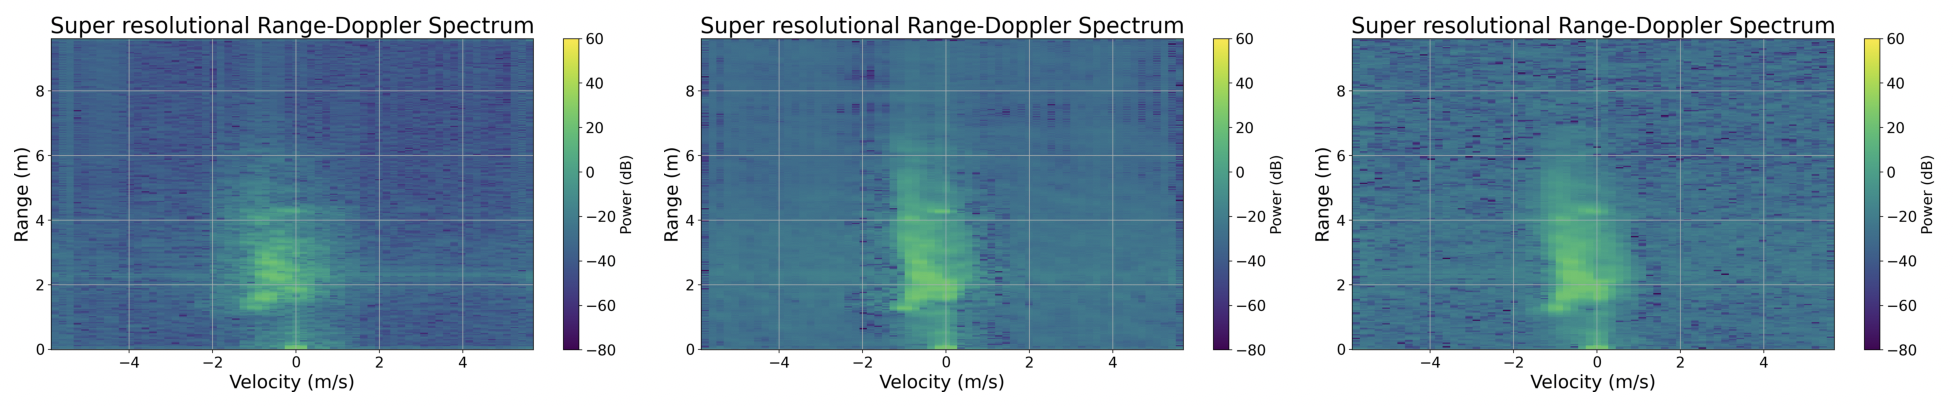
\includegraphics[scale=.45]{figures/evaluation_processing_mse_A.png}
    \caption{Super-resolution range-Doppler maps of different types of the input data representation, from left to right real and imaginary representation, amplitude representation as well as amplitude and phase representation, respectively.}
    \label{Super-resolution images of the separation types}
\end{figure}

Analyzed from the results, since the visualization of range-Doppler map is affected by amplitude, it is beneficial to use amplitude for training. From the perspective of evaluation losses, training with only amplitude is the best. However, since it loses the information of phase, and the amplitude and phase representation type is mostly better than real and imaginary representation type in terms of the evaluation losses and visual effect, the amplitude and phase representation type will be maintained in the subsequent evaluations.

\begin{spacing}{1.5}
\textbf{\large{Dimension processing types}}
\end{spacing}
Operated by the \gls{rfft}, the shape along the range axis turns to an prime value, which will affect both the Transformer division and the downsampling process. However, since there is no downsampling operation and segmentation along the axes in the \gls{dp}-\gls{tf} Transformer model, it can still run normally without additional dimension processing. Therefore, there are three dimensional processing types: no processing, padding, and convolution. Based on the amplitude and phase representation type and keeping other settings unchanged, the loss metrics in Table \ref{Evaluation losses of the dimension processing types comparison} and the super-resolution range-Doppler maps in Figure \ref{super-resolution images of the dimension processing types} are obtained.

\begin{table}
    \centering
    \caption{Evaluation losses of different dimension processing types, where B1 represents no processing type, B2 is the padding and B3 denotes the convolutional layer as the processing type.}
    \label{Evaluation losses of the dimension processing types comparison}
    \begin{tabular}{l|c|c|c|c|c}
        \hline
        Dimension processing & MSE & SDR & LSD & WMSE & Perceptual \\
        \hline
        B1 & 3.100 & -6.312 & 0.427 & 0.194 & 19.081 \\
        \hline
        B2 & 3.113 & \textbf{-6.611} & \textbf{0.420} & \textbf{0.190} & 19.092 \\
        \hline
        B3 & \textbf{2.349} & -5.908 & 0.451 & 0.206 & \textbf{16.259} \\
        \hline
    \end{tabular}
\end{table}

\begin{figure}
    \centering
    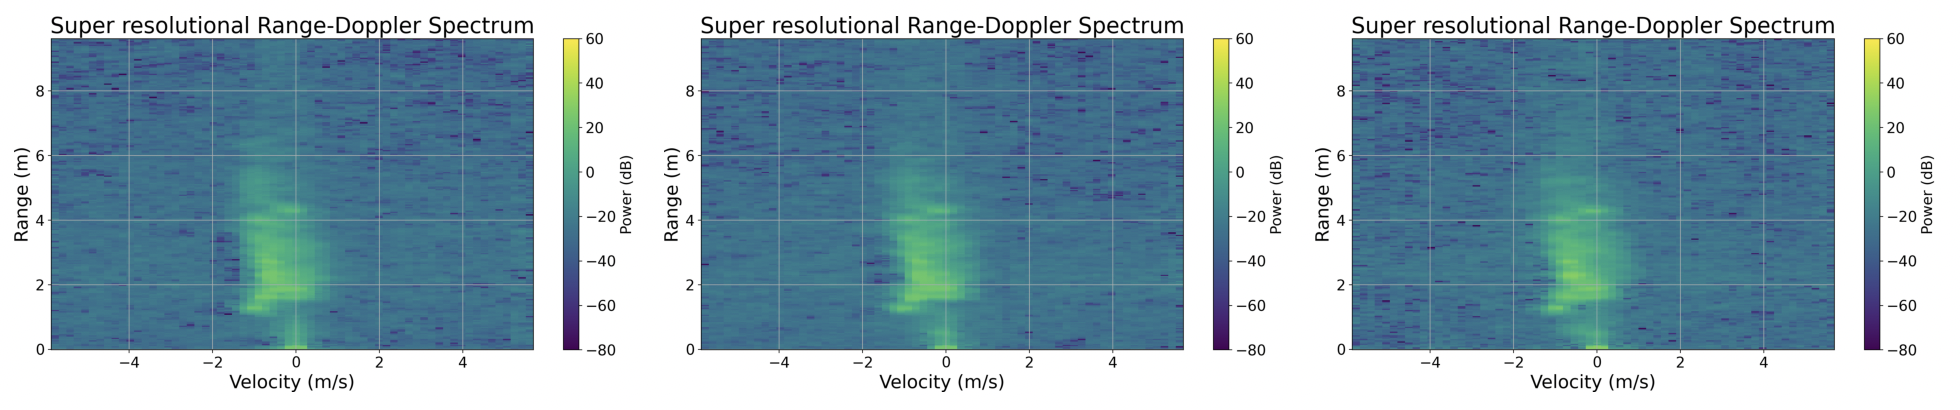
\includegraphics[scale=.45]{figures/evaluation_processing_mse_B.png}
    \caption{Super-resolution range-Doppler maps of different dimension processing types, from left to right no processing, padding and convolution layer, respectively}
    \label{super-resolution images of the dimension processing types}
\end{figure}

While the convolutional layer as the dimension processing type leads to more parameters, the padding processing type can still obtain a better result in multiple evaluation losses. The reason could be that using convolution layer to remove a dimension along the range axis may result in information loss. Subsequent evaluations will be based on the padding dimension processing type.

\begin{spacing}{1.5}
\textbf{\large{Upsampling types}}
\end{spacing}
The two most common upsampling methods are transposed convolutional layer and pixel shuffle approach. The block, containing transposed convolutional layer, \gls{ln} and \gls{relu} activation function, will result in a lot of new parameters, while the pixel shuffle operation does not generate any new parameters. Table \ref{Evaluation losses of the upsampling types comparison} and Figure \ref{super-resolution images of the upsampling types} show the performance of two approaches in terms of evaluation losses and super-resolution range-Doppler maps.

Although the transposed convolutional layer brings a large number of new parameters, it does not surpass pixel shuffle layer in all loss metrics, especially the perceptual loss is higher. Visually, the right range-Doppler map in Figure \ref{super-resolution images of the upsampling types} is even more reasonable for the dynamic range part. Therefore, the pixel shuffle layer will be used as the upsampling type in the subsequent evaluations.

\begin{table}
    \centering
    \caption{Evaluation losses of different upsampling types, where C1 represents the transposed convolutional layer and C2 denotes the pixel shuffle approach as the upsampling layer.}
    \label{Evaluation losses of the upsampling types comparison}
    \begin{tabular}{l|c|c|c|c|c|c}
        \hline
        Upsampling types & \#Params & MSE & SDR & LSD & WMSE & Perceptual \\
        \hline
        C1 & 113,866 & 3.113 & \textbf{-6.611} & \textbf{0.420} & \textbf{0.190} & 19.092 \\
        \hline
        C2 & 48,042 & \textbf{2.560} & -4.206 & 0.506 & 0.269 & \textbf{17.918} \\
        \hline
    \end{tabular}
\end{table}

\begin{figure}
    \centering
    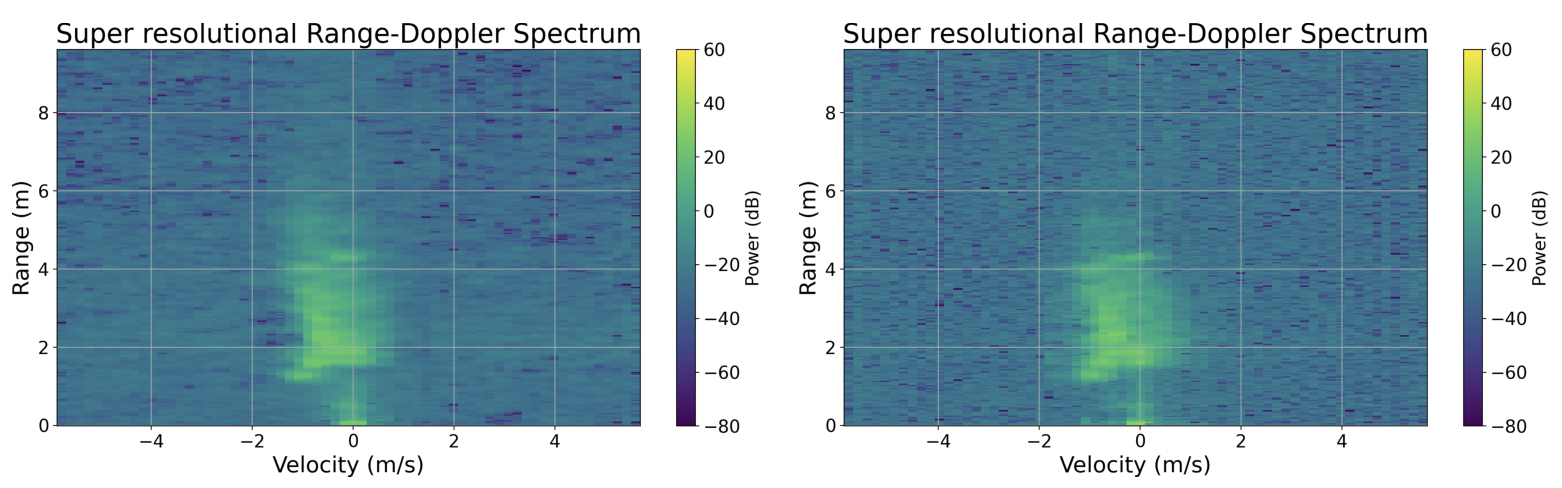
\includegraphics[scale=.45]{thesis/figures/evaluation_processing_C.png}
    \caption{Super-resolution range-Doppler maps of different upsampling types, left using the transposed convolutional layer and right with the pixel shuffle layer.}
    \label{super-resolution images of the upsampling types}
\end{figure}


\begin{spacing}{1.5}
\textbf{\large{Logarithm types}}
\end{spacing}
When the amplitude is part of the input, the range of the amplitude will affect the learning process, causing it to focus more on areas with higher signal power and ignore the loss caused by areas with less amplitude. Therefore, in this evaluation, the impact of the logarithm operation will be evaluated.

\begin{table}
    \centering
    \caption{Evaluation losses of the effect of the logarithm, where D1 represents no logarithm operation, D2 uses the base 10 logarithm operation. Accordingly, the \gls{mse} training loss in D1 case uses the amplitude in linear scale while in D2 uses the logarithmic amplitude.}
    \label{Evaluation losses of the logarithm types comparison}
    \begin{tabular}{l|c|c|c|c|c}
        \hline
        Logarithm types & MSE & SDR & LSD & WMSE & Perceptual \\
        \hline
        D1 & 2.560 & -4.206 & 0.506 & 0.269 & 17.918 \\
        \hline
        D2 & \textbf{1.740} & \textbf{-9.251} & \textbf{0.295} & \textbf{0.130} & \textbf{17.636} \\
        \hline
    \end{tabular}
\end{table}

\begin{figure}
    \centering
    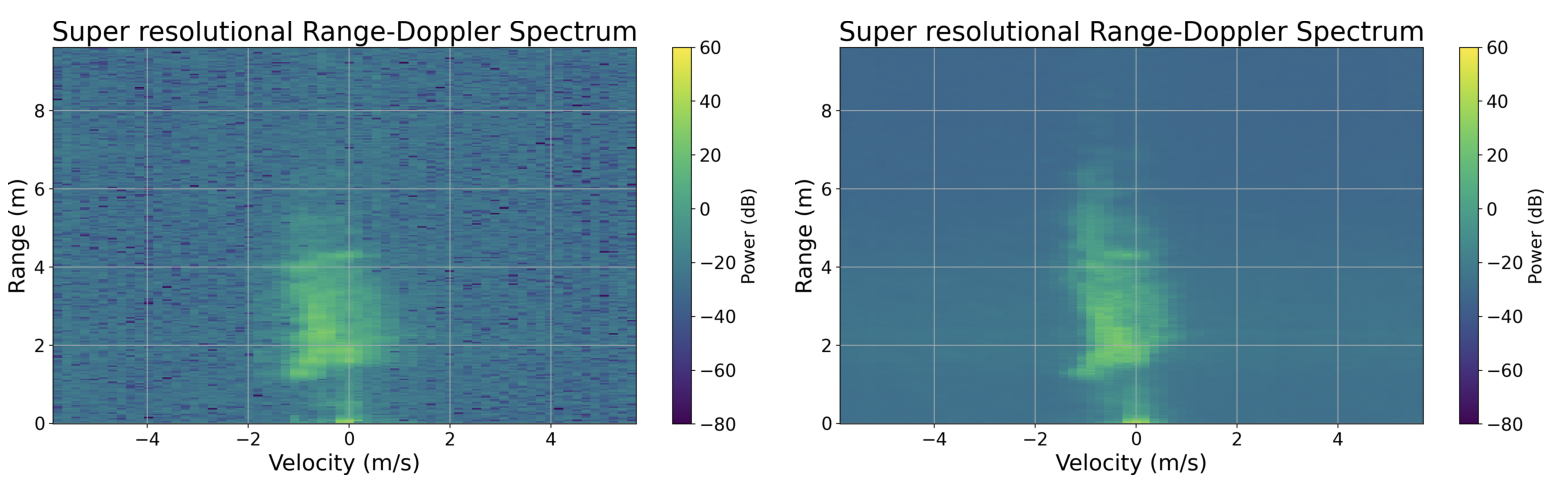
\includegraphics[scale=.45]{figures/evaluation_processing_D.png}
    \caption{Super-resolution range-Doppler maps of the cases without logarithm and with logarithm operation, from left to right, respectively.}
    \label{super-resolution images of the logarithm types}
\end{figure}

From Table \ref{Evaluation losses of the logarithm types comparison}, it can be clearly seen that after using the logarithm operation with base 10, significant improvements have been achieved in all evaluation losses. However, compared with the left range-Doppler map in Figure \ref{super-resolution images of the logarithm types}, the right super-resolution range-Doppler map has a blurring effect in the background. The reason would be that in the left range-Doppler map the model pays less attention on the low amplitude signal as well as the noise and uses smaller values instead. After using the logarithm, the signals with low amplitude get more attention while the noise is still hard to learn, so that the noise is mostly predicted as relatively low amplitude and then look blurry.

\begin{spacing}{1.5}
\textbf{\large{Amplitude normalization types}}
\end{spacing}
Similar to the idea of logarithm operation, the normalization operation can reduce the dynamic range of the data. According to the maximum and minimum values of each dataset, the amplitude of each dataset can be accordingly converted to the range of (-1, 1) or (0, 1) . In addition, it can also be not normalized. Furthermore, since the normalization will result in a small gradient, the learning rate is tuned by the cases, only the case without normalization uses the learning rate as 1e-5, otherwise the learning rate as 1e-3. The results of the evaluation losses and the super-resolution range-Doppler maps are shown in Table \ref{Evaluation losses of the amplitude normalization types comparison in the case of no angle normalization} and Figure \ref{evaluation processing E} respectively.

\begin{table}
    \centering
    \caption{Evaluation losses of different amplitude normalization types, where E1 represent no normalization operation, E2 is in the range of (-1, 1), E3 denotes in the range of (0,1).}
    \label{Evaluation losses of the amplitude normalization types comparison in the case of no angle normalization}
    \begin{tabular}{l|c|c|c|c|c}
        \hline
        Amplitude normalization & MSE & SDR & LSD & WMSE & Perceptual \\
        \hline
        E1 & 1.740 & \textbf{-9.251} & \textbf{0.295} & 0.130 & 17.636 \\
        \hline
        E2 & 1.711 & -6.841 & 0.349 & \textbf{0.108} & 14.770 \\
        \hline
        E3 & \textbf{1.073} & -6.327 & 0.358 & 0.119 & \textbf{14.639} \\
        \hline
    \end{tabular}
\end{table}

\begin{figure}
    \centering
    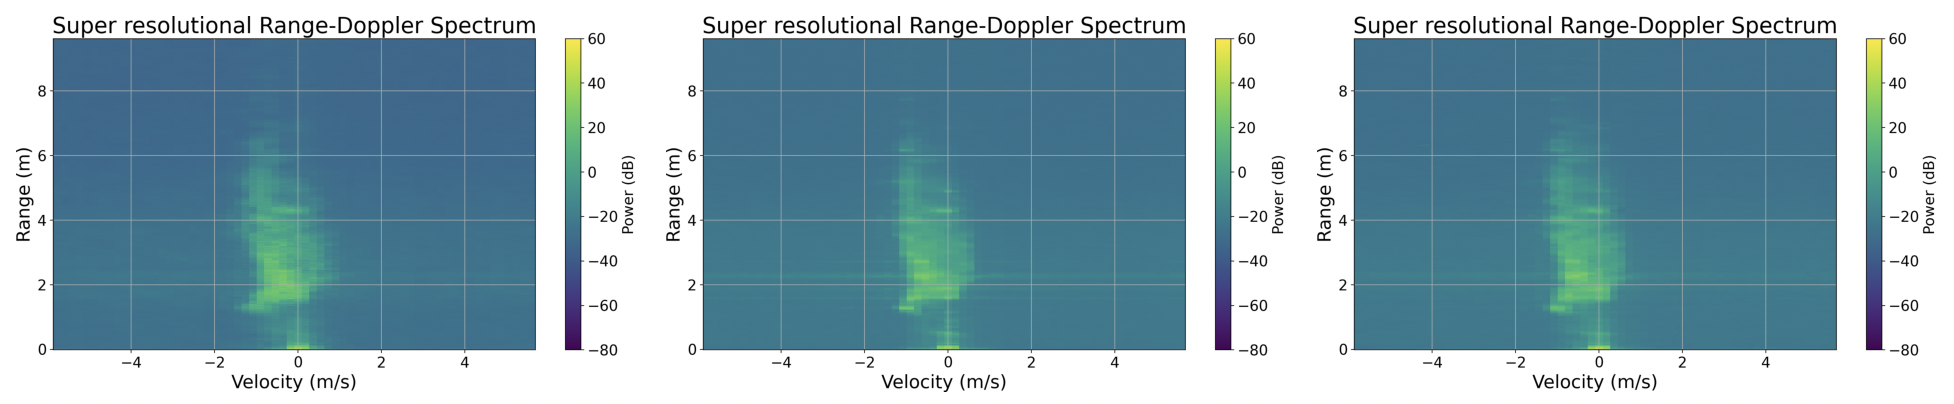
\includegraphics[scale=.45]{figures/evaluation_processing_E.png}
    \caption{Super-resolution range-Doppler maps of different amplitude normalization types, from left to right, no amplitude normalization, normalization in (-1, 1) and normalization in (0, 1), respectively.}
    \label{evaluation processing E}
\end{figure}

In general, the introduction of the normalization operation is conducive to reduce multiple evaluation losses, among which the optimization of perceptual loss is the most obvious, which represents visual optimization, since the \gls{vgg} expects the normalized input, ideally in the (0, 1) range. The normalization in (0, 1) form obtains the most balanced result, so the amplitude normalization will be kept in the range of (0, 1) in subsequent evaluations.

\begin{spacing}{1.5}
\textbf{\large{Angle normalization types}}
\end{spacing}
In the amplitude and phase representation type, in addition to the amplitude being normalized, the angle can also be normalized and converted to (-1, 1) divided by  $\mathrm{\pi}$. The results are shown in Table \ref{Evaluation losses of the angle normalization types comparison} and Figure \ref{evaluation processing F}.

From the results, the normalization of the angle doesn't bring much improvement in the most evaluation losses. The reason is that the angle itself is within the range of (-$\mathrm{\pi}$, $\mathrm{\pi}$), and its dynamic range is not that large as amplitude. Therefore, the normalization operation will not cause many differences.

\begin{table}
    \centering
    \caption{Evaluation losses of the effect of the angle normalization type, where F1 represent no angle normalization operation, F2 denotes the angle normalization in the range of (-1, 1).}
    \label{Evaluation losses of the angle normalization types comparison}
    \begin{tabular}{l|c|c|c|c|c}
        \hline
        Angle normalization & MSE & SDR & LSD & WMSE & Perceptual \\
        \hline
        F1 & \textbf{1.073} & \textbf{-6.327} & \textbf{0.358} & 0.119 & \textbf{14.639} \\
        \hline
        % F2 & 1.154 & \textbf{-6.814} & \textbf{0.349} & \textbf{0.115} & \textbf{14.607} \\
        % \hline
        F2 & 1.330 & -6.068 & 0.363 & \textbf{0.117} & 15.204 \\
        \hline
    \end{tabular}
\end{table}

\begin{figure}
    \centering
    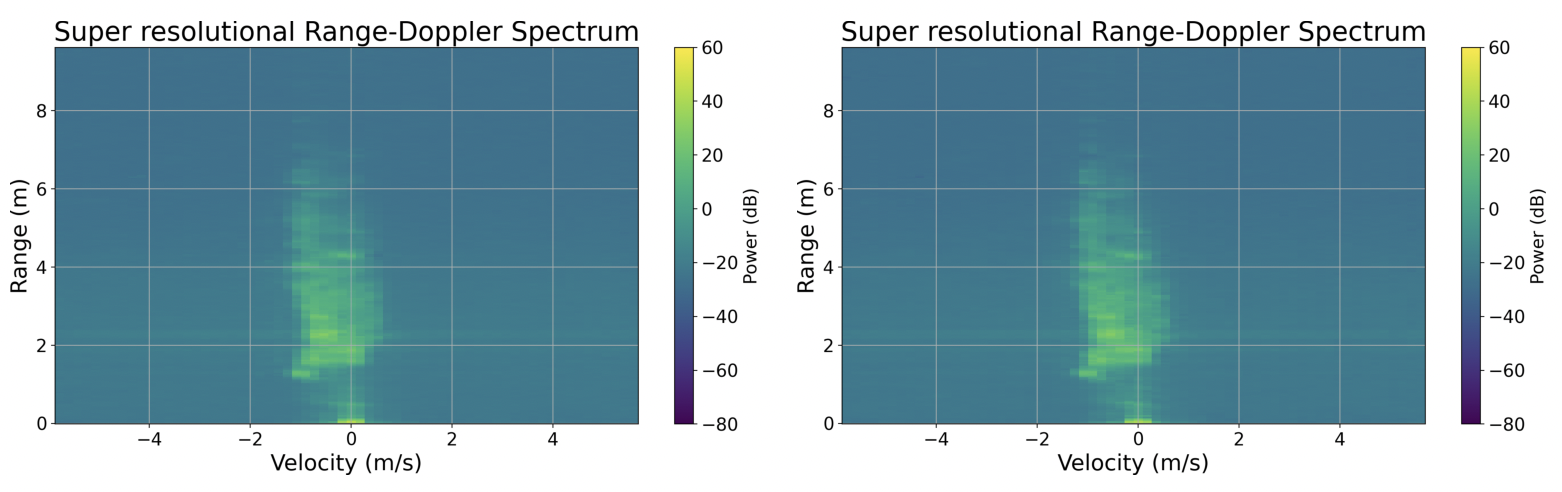
\includegraphics[scale=.45]{thesis/figures/evaluation_processing_F_new.png}
    \caption{Super-resolution range-Doppler maps of the effect of the angle normalization type, left without angle normalization and right with angle normalization.}
    \label{evaluation processing F}
\end{figure}

In conclusion, based on the above evaluations and analysis, the combination of processing methods tends to use padding for dimensional processing, pixel shuffle approach as the upsampling type, amplitude and phase representation determined as the conversion of the complex-valued data, logarithm operation and normalization operation in the range of (0, 1) on the amplitude, but no additional normalization operation performed on the phase.

\section{Training loss functions} \label{training loss functions evaluations}
Different from the evaluation loss functions, there are six types of training loss functions. Based on the optimal combination of the processing methods combination obtained in the section \ref{processing methods comparisons} and \gls{dp}-\gls{tf} Transformer model, different training loss functions are used to train the model, so as to obtain one training loss function that is most suitable for the range-Doppler map upsampling task. The hyperparameters such as the ratio $\lambda$ between the amplitude loss and angle loss in the training loss function and learning rate will be adjusted according to their values according to a few batches at the very beginning. In addition, \gls{sdr} and perceptual loss functions require a pretraining phase by the \gls{lsd} training loss function, since they are not stable in the early stage. Table \ref{Evaluation losses of the training loss functions comparison} and Figure \ref{training loss functions comparison} are the results obtained by different training loss functions.


\begin{table}
    \centering
    \caption{Evaluation losses of different training loss functions, horizontal axis is the evaluation loss functions, vertical axis is the training loss functions.}
    \label{Evaluation losses of the training loss functions comparison}
    \begin{tabular}{l|c|c|c|c|c}
        \hline
        Loss comparison & MSE & SDR & LSD & WMSE & Perceptual \\
        \hline
        MSE & \textbf{1.073} & -6.327 & 0.358 & 0.119 & 14.639 \\
        \hline
        SDR & 1.110 & -5.683 & 0.370 & 0.121 & 14.163 \\
        \hline
        LSD & 1.232 & \textbf{-6.736} & \textbf{0.351} & \textbf{0.108} & 14.198 \\
        \hline
        PLSD & 1.424 & -6.434 & 0.356 & 0.124 & 16.999 \\
        \hline
        WMSE & 1.279 & -5.967 & 0.365 & 0.131 & 17.478 \\
        \hline
        Perceptual & 6.174 & -4.129 & 0.417 & 0.393 & \textbf{13.882} \\
        \hline
    \end{tabular}
\end{table}

\begin{figure}
    \centering
    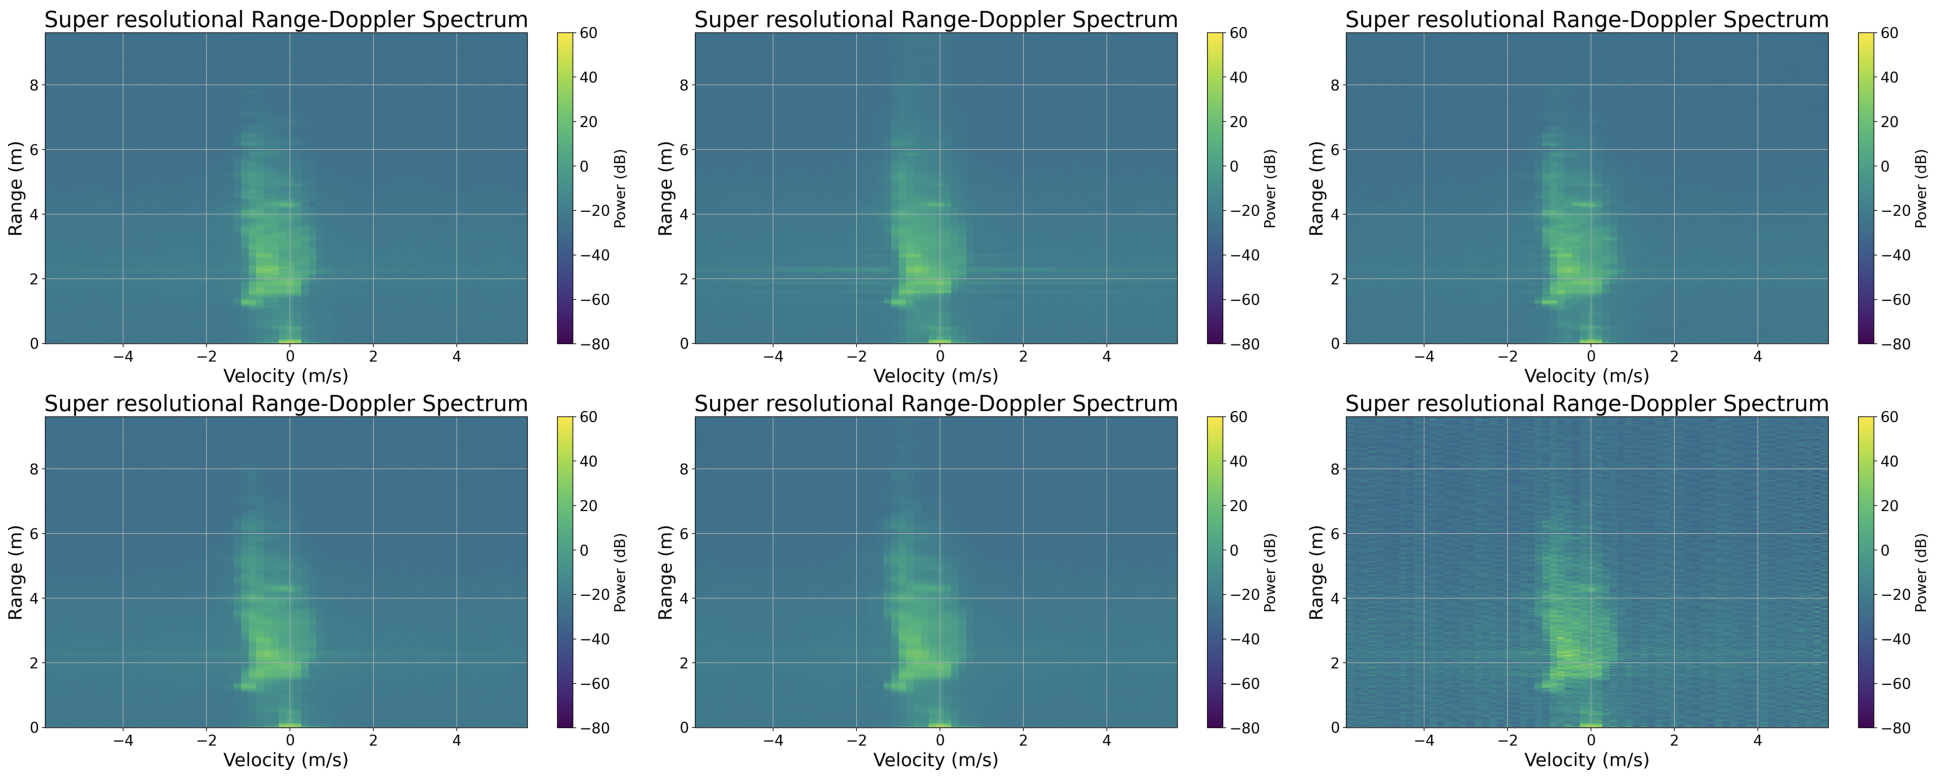
\includegraphics[scale=.4]{thesis/figures/evaluation_loss_functions.png}
    \caption{Super-resolution range-Doppler maps of different training loss functions, in the first row from left to right MSE, SDR and LSD, in the second row from left to right PLSD, WMSE and perceptual loss functions.}
    \label{training loss functions comparison}
\end{figure}

From the results, it can be seen that the \gls{lsd} training loss function can obtain better results in most of the evaluation losses, but from the visual perspective of super-resolution range-Doppler maps, the range-Doppler maps trained by perceptual loss effectively eliminate the blurring problem, that is, the amplitude difference in the background can be seen. Therefore, the training loss function \gls{lsd} can be combined with the perceptual loss to take advantage of both pros.

\begin{spacing}{1.5}
\textbf{\large{Loss combination}}
\end{spacing} 
According to the loss combination as written in formula \ref{loss combination equation}, the relationship $\lambda_c$ between \gls{lsd} and perceptual loss should be determined. We compare a few loss values of the early batches and make sure that the main loss value comes from the \gls{lsd} loss but still influenced by the perceptual loss to a certain content, then Table \ref{Evaluation losses of the training loss functions combination comparison} and Figure \ref{lsd+perceptual combination} are obtained.

\begin{table}
    \centering
    \caption{Evaluation losses of the training loss combination with different ratios.}
    \label{Evaluation losses of the training loss functions combination comparison}
    \begin{tabular}{l|c|c|c|c|c}
        \hline
        LSD combination & MSE & SDR & LSD & WMSE & Perceptual \\
        \hline
        Lambda=1 & 2.464 & -5.270 & 0.383 & 0.220 & 13.779 \\
        \hline
        Lambda=0.5 & 1.731 & -5.375 & 0.380 & 0.179 & \textbf{12.320 }\\
        \hline
        Lambda=1e-1 & 1.347 & -5.829 & 0.369 & 1.150 & 12.979 \\
        \hline
        Lambda=1e-2 & 1.288 & -6.514 & 0.355 & 0.116 & 13.213 \\
        \hline
        Lambda=1e-3 & 1.486 & \textbf{-7.268} & \textbf{0.341} & \textbf{0.108} & 13.729 \\
        \hline
        Lambda=1e-4 & \textbf{1.265} & -6.405 & 0.357 & 0.115 & 14.138 \\
        \hline
    \end{tabular}
\end{table}

\begin{figure}
    \centering
    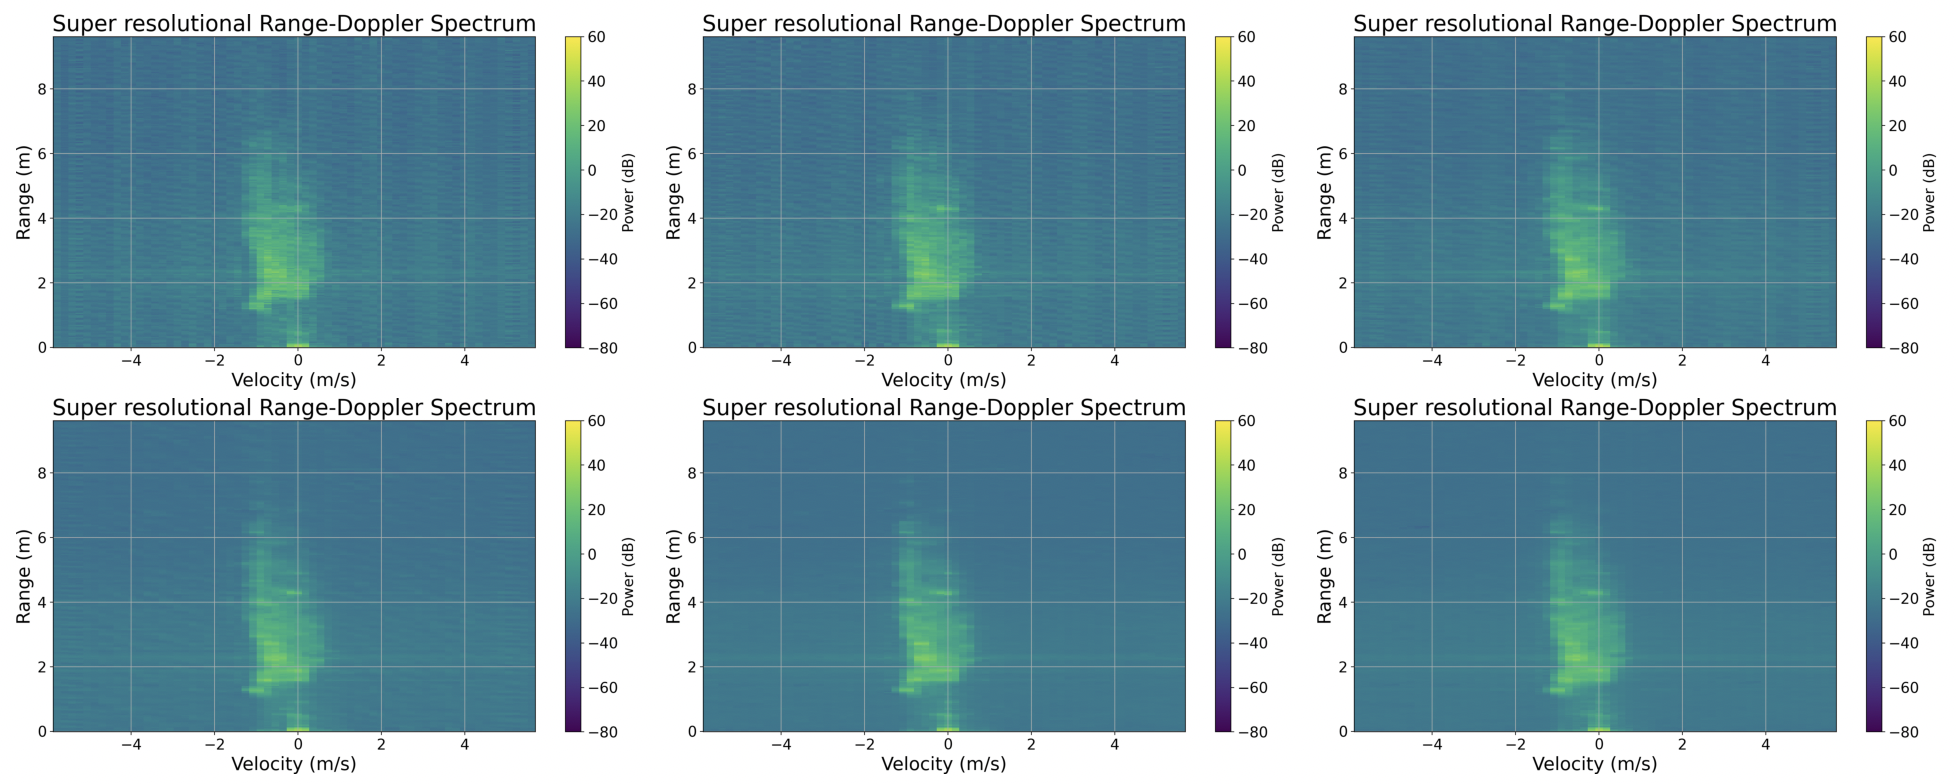
\includegraphics[scale=.45]{figures/evaluation_loss_combination.png}
    \caption{Super-resolution range-Doppler maps of the training loss combination with different ratios, in the first row from left to right are lambda as 1, 0.5 and 0.1, while in the second row from left to right 1e-2, 1e-3, 1e-4.}
    \label{lsd+perceptual combination}
\end{figure}

The overall relationship between the \gls{lsd} loss function and perceptual loss function is that with the importance of the perceptual loss increasing in the loss combination, the evaluation perceptual loss decreases while the other evaluation losses is increasing. Since the loss combination is going to optimize the perceptual loss, the hyperparameter $\lambda_C$ is determined as 0.5, that is, the training loss function written as
\begin{equation}
    \centering
    \mathcal{L}_{\text{Combination}} = \mathcal{L}_{\text{LSD}} + 0.5 \times \mathcal{L}_{\text{Perceptual}}.
    \label{loss combination}
\end{equation}


\section{cGAN comparison} \label{cGAN comparison}
With the mutual supervision of the generator and discriminator, the output of generator can be visually more pleasing. Therefore, in this section, the \gls{cgan} model is evaluated, the generator keeps using the \gls{dp}-\gls{tf} Transformer model, and target training loss function is the loss combination from section \ref{training loss functions evaluations}. The generator loss is denoted as
\begin{equation}
    \centering
    \mathcal{L}_{\text{Gen}} = \mathcal{L}_{\text{LSD}} + 0.5 \times \mathcal{L}_{\text{Perceptual}} + \lambda_g \times \mathcal{L}_{\text{GAN, Gen}},
    \label{loss combination}
\end{equation}

where $\lambda_g$ is going to be tuned. Furthermore, as said in section \ref{discriminator}, the discriminator has two types, no low-resolution range-Doppler maps or with low-resolution range-Doppler maps as input. Therefore, both cases have been evaluated, where Table \ref{Evaluation losses of the cGAN model comparison in the case of discriminator without low-resolution image as input} and Figure \ref{Super-resolution images of the cGAN model no low-res} show the results in the case of the discriminator without any low-resolution information while Table \ref{Evaluation losses of the cGAN model comparison in the case of discriminator with low-resolution image as input} and Figure \ref{Super-resolution images of the cGAN model with low-res} are the results given the low-resolution range-Doppler maps.

\begin{table}
    \centering
    \caption{Evaluation losses of the adversarial loss combination with different ratios in the case of the discriminator without low-resolution range-Doppler maps as input.}
    \label{Evaluation losses of the cGAN model comparison in the case of discriminator without low-resolution image as input}
    \begin{tabular}{l|c|c|c|c|c}
        \hline
        cGAN & MSE & SDR & LSD & WMSE & Perceptual \\
        \hline
        $\lambda_g$=5e-1 & 1.802 & -5.216 & 0.383 & 0.186 & 13.543 \\
        \hline
        $\lambda_g$=1e-1 & 1.621 & -5.183 & 0.384 & 0.172 & 12.898 \\
        \hline
        $\lambda_g$=5e-2 & \textbf{1.447} & -5.463 & 0.379 & 0.181 & 13.311 \\
        \hline
        $\lambda_g$=1e-2 & 1.640 & -5.690 & 0.374 & \textbf{0.169} & \textbf{11.881} \\
        \hline
        $\lambda_g$=5e-3 & 1.525 & -5.305 & 0.382 & 0.193 & 12.956 \\
        \hline
        $\lambda_g$=1e-3 & 2.072 & \textbf{-5.845} & \textbf{0.370} & 0.182 & 14.396 \\
        \hline
    \end{tabular}
\end{table}

\begin{figure}
    \centering
    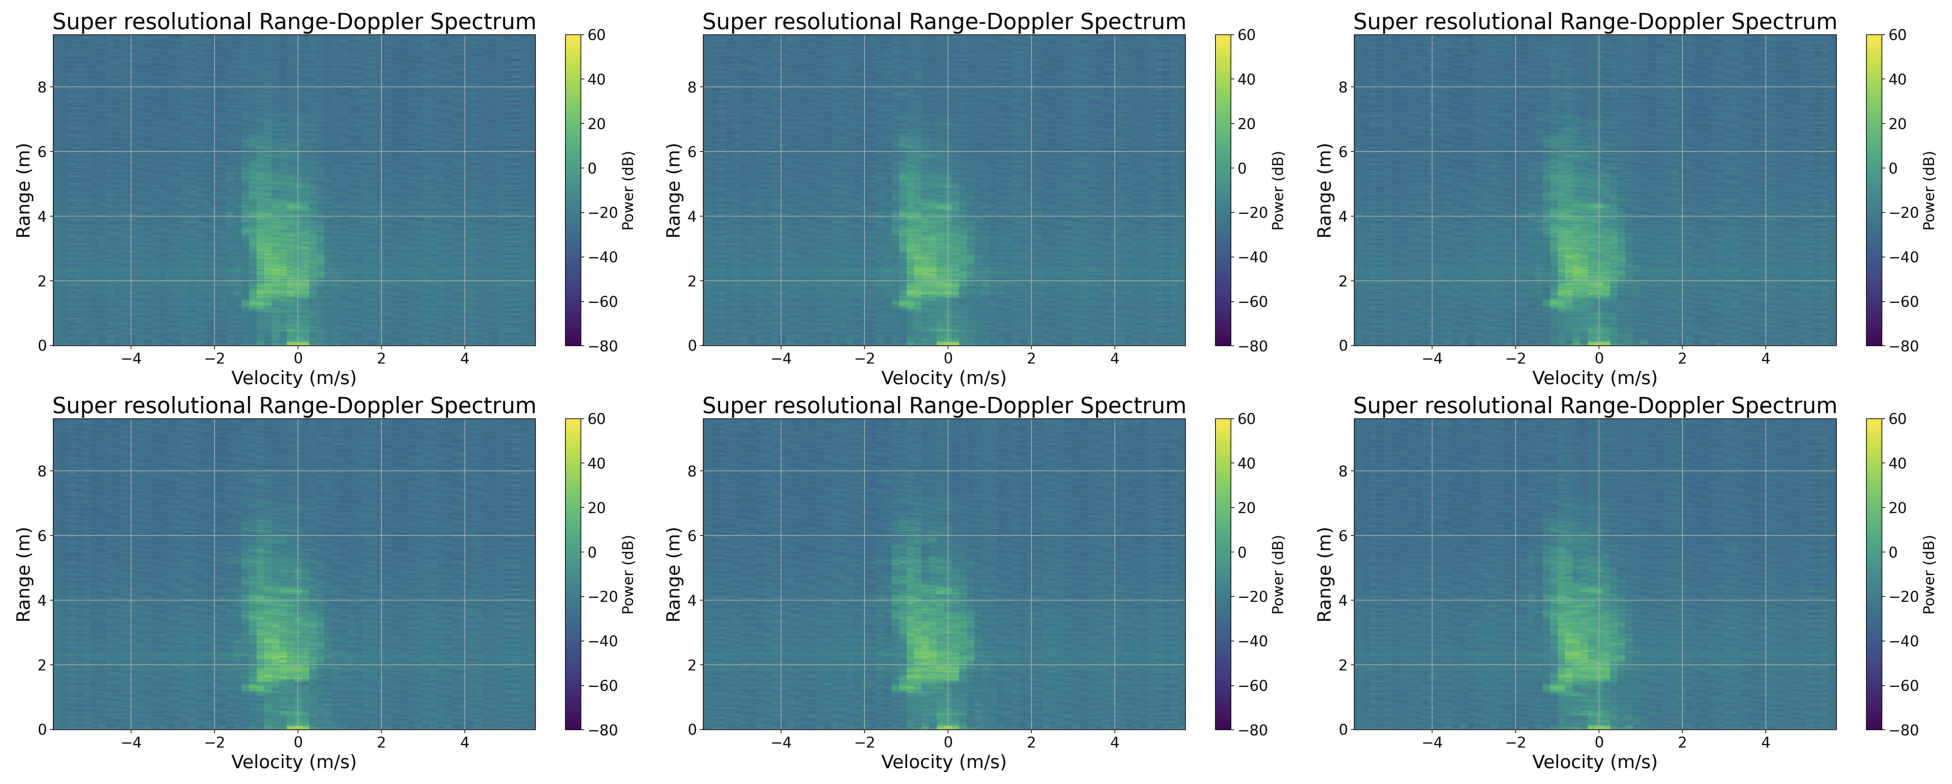
\includegraphics[scale=.45]{thesis/figures/evaluation_cGAN_no_low_res.png}
    \caption{Super-resolution range-Doppler maps of the adversarial loss combination with different ratios in the case of the discriminator without low-resolution range-Doppler maps as input, in the first row from left to right are $\lambda_g$ as 5e-1, 1e-1 and 5e-2, while in the second row from left to right 1e-2, 5e-3, 1e-3.}
    \label{Super-resolution images of the cGAN model no low-res}
\end{figure}

It can be seen that \gls{cgan} model is able to improve the perceptual loss, no matter with or without the low-resolution range-Doppler map. Both cases are better, especially when the adversarial loss ratio sets as 1e-2, whereas the discriminator without the low-resolution range-Doppler map gets a relatively better perceptual evaluation loss. The reason could be that the concatenating operation of the low-resolution and high(super)-resolution range-Doppler map would confuse the discriminator, that is, the discriminator focuses more on the mapping relationship between low- and super-resolution range-Doppler map, rather than on the super-resolution range-Doppler map itself, and additionally, the loss calculation in the perceptual loss has no inputs of the low-resolution range-Doppler map. Perhaps the comparison directly between the super- and high-resolution range-Doppler maps is simple for the discriminator rather than with the low-resolution range-Doppler map as the medium. In conclusion, the discriminator without low-resolution range-Doppler map will be used and the generator loss turns to be

\begin{equation}
    \centering
    \mathcal{L}_{\text{Gen}} = \mathcal{L}_{\text{LSD}} + 0.5 \times \mathcal{L}_{\text{Perceptual}} + 0.01 \times \mathcal{L}_{\text{GAN, Gen}}.
    \label{loss combination}
\end{equation}


\begin{table}[!htp]
    \centering
    \caption{Evaluation losses of the adversarial loss combination with different ratios in the case of the discriminator with low-resolution range-Doppler maps as input, where the number of parameters of the generator is 48,042 while that of the discriminator is 76,267.}
    \label{Evaluation losses of the cGAN model comparison in the case of discriminator with low-resolution image as input}
    \begin{tabular}{l|c|c|c|c|c}
        \hline
        cGAN & MSE & SDR & LSD & WMSE & Perceptual \\
        \hline
        $\lambda_g$=1e-1 & 1.592 & -5.361 & 0.381 & 0.164 & 13.861 \\
        \hline
        $\lambda_g$=5e-2 & 1.491 & -5.628 & \textbf{0.374} & \textbf{0.158} & 12.126 \\
        \hline
        $\lambda_g$=1e-2 & \textbf{1.339} & -5.103 & 0.385 & 0.177 & \textbf{11.926} \\
        \hline
        $\lambda_g$=5e-3 & 1.628 & -5.461 & 0.379 & 0.165 & 13.511 \\
        \hline
        $\lambda_g$=1e-3 & 1.920 & \textbf{-5.648} & 0.375 & 0.159 & 13.257 \\
        \hline
        $\lambda_g$=1e-4 & 3.593 & -5.331 & 0.381 & 0.190 & 14.148 \\
        \hline
    \end{tabular}
\end{table}

\begin{figure}[!htp]
    \centering
    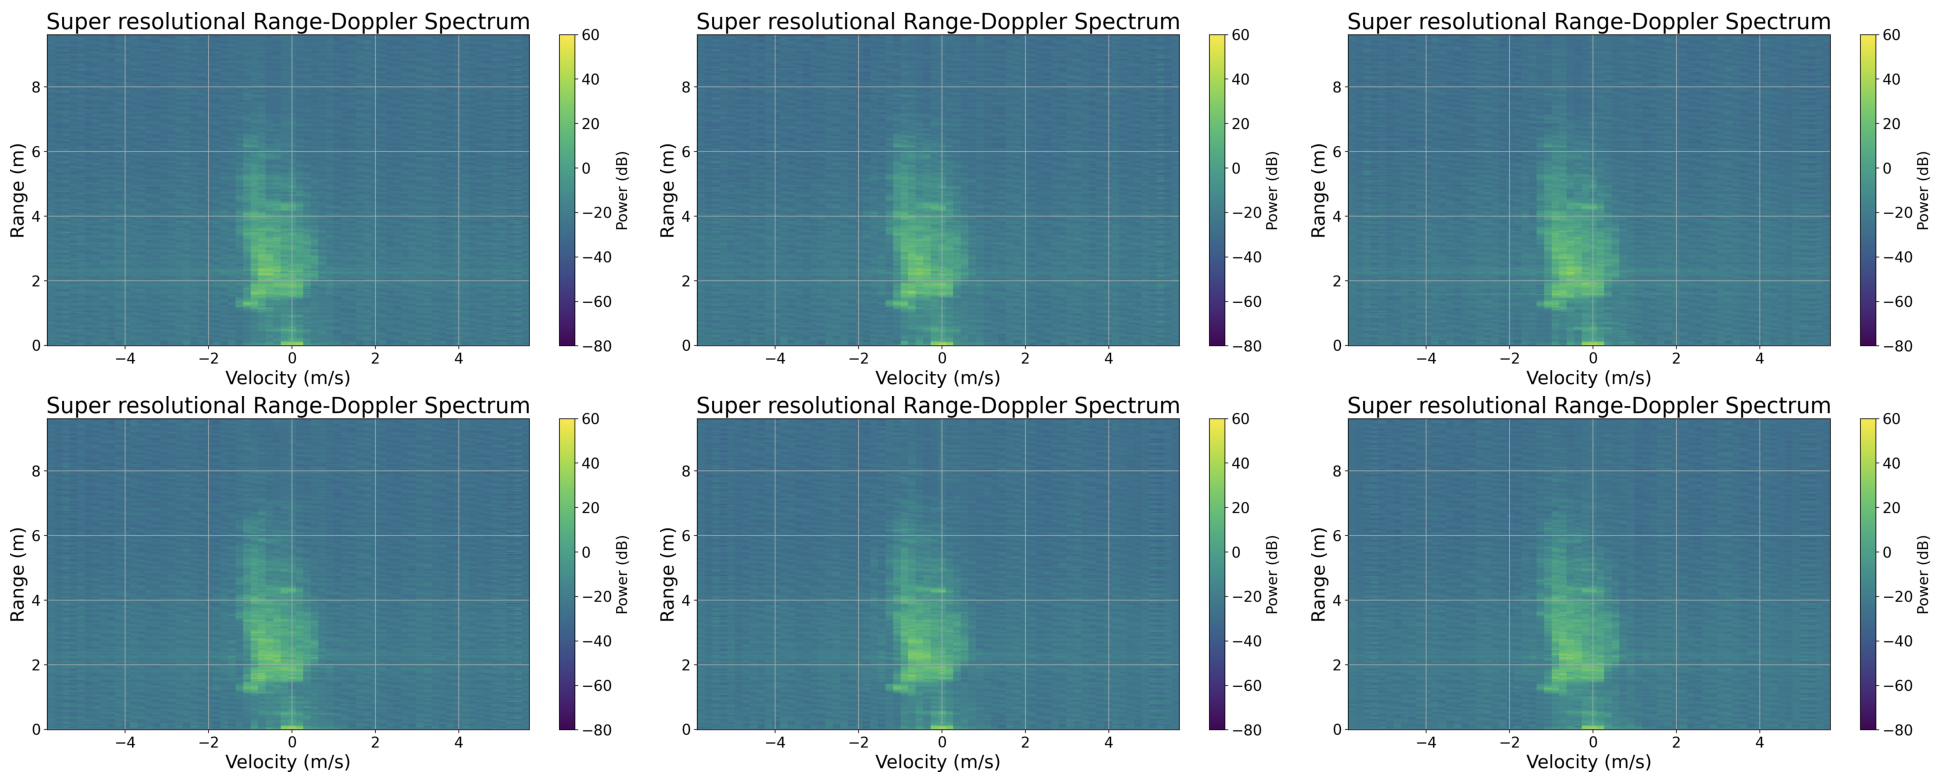
\includegraphics[scale=.45]{thesis/figures/evaluation_cGAN_with_low_res.png}
    \caption{Super-resolution range-Doppler maps of the adversarial loss combination with different ratios in the case of the discriminator with low-resolution range-Doppler maps as input, in the first row from left to right are $\lambda_g$ as 1e-1, 5e-2 and 1e-2, while in the second row from left to right 5e-3, 1e-3 and 1e-4.}
    \label{Super-resolution images of the cGAN model with low-res}
\end{figure}


\section{VGG layers in the perceptual loss} \label{vgg layers comparison}
In this section, different combinations of the \gls{vgg} layers are evaluated, by default the last convolutional layers of the first four blocks are used. Table \ref{Evaluation losses of different VGG layers} and Figure \ref{Super-resolution images of different VGG layers} show the results trained by the loss combination with different \gls{vgg} layers used. With the deeper layer to be used, many evaluation losses decrease. However, in order to improve the perceptual loss, the default combination is still better one.

\begin{table}[!htp]
    \centering
    \caption{Evaluation losses of different combinations of the VGG layers in the training loss combination.}
    \label{Evaluation losses of different VGG layers}
    \begin{tabular}{l|c|c|c|c|c}
        \hline
        VGG layers comparison & MSE & SDR & LSD & WMSE & Perceptual \\
        \hline
        b1c2+b2c2+b3c4 & 1.975 & -5.366 & 0.380 & 0.167 & 12.793 \\
        \hline
        b1c2+b2c2+b3c4+b4c4 & 1.731 & -5.375 & 0.380 & 0.179 & \textbf{12.320} \\
        \hline
        b1c2+b2c2+b3c4+b4c4+b5c4 & 1.731 & \textbf{-6.082} & \textbf{0.366} & \textbf{0.157} & 13.714 \\
        \hline
        b2c2+b3c4+b4c4 & \textbf{1.730} & -5.530 & 0.379 & 0.186 & 14.857 \\
        \hline
    \end{tabular}
\end{table}

\begin{figure}[!htp]
    \centering
    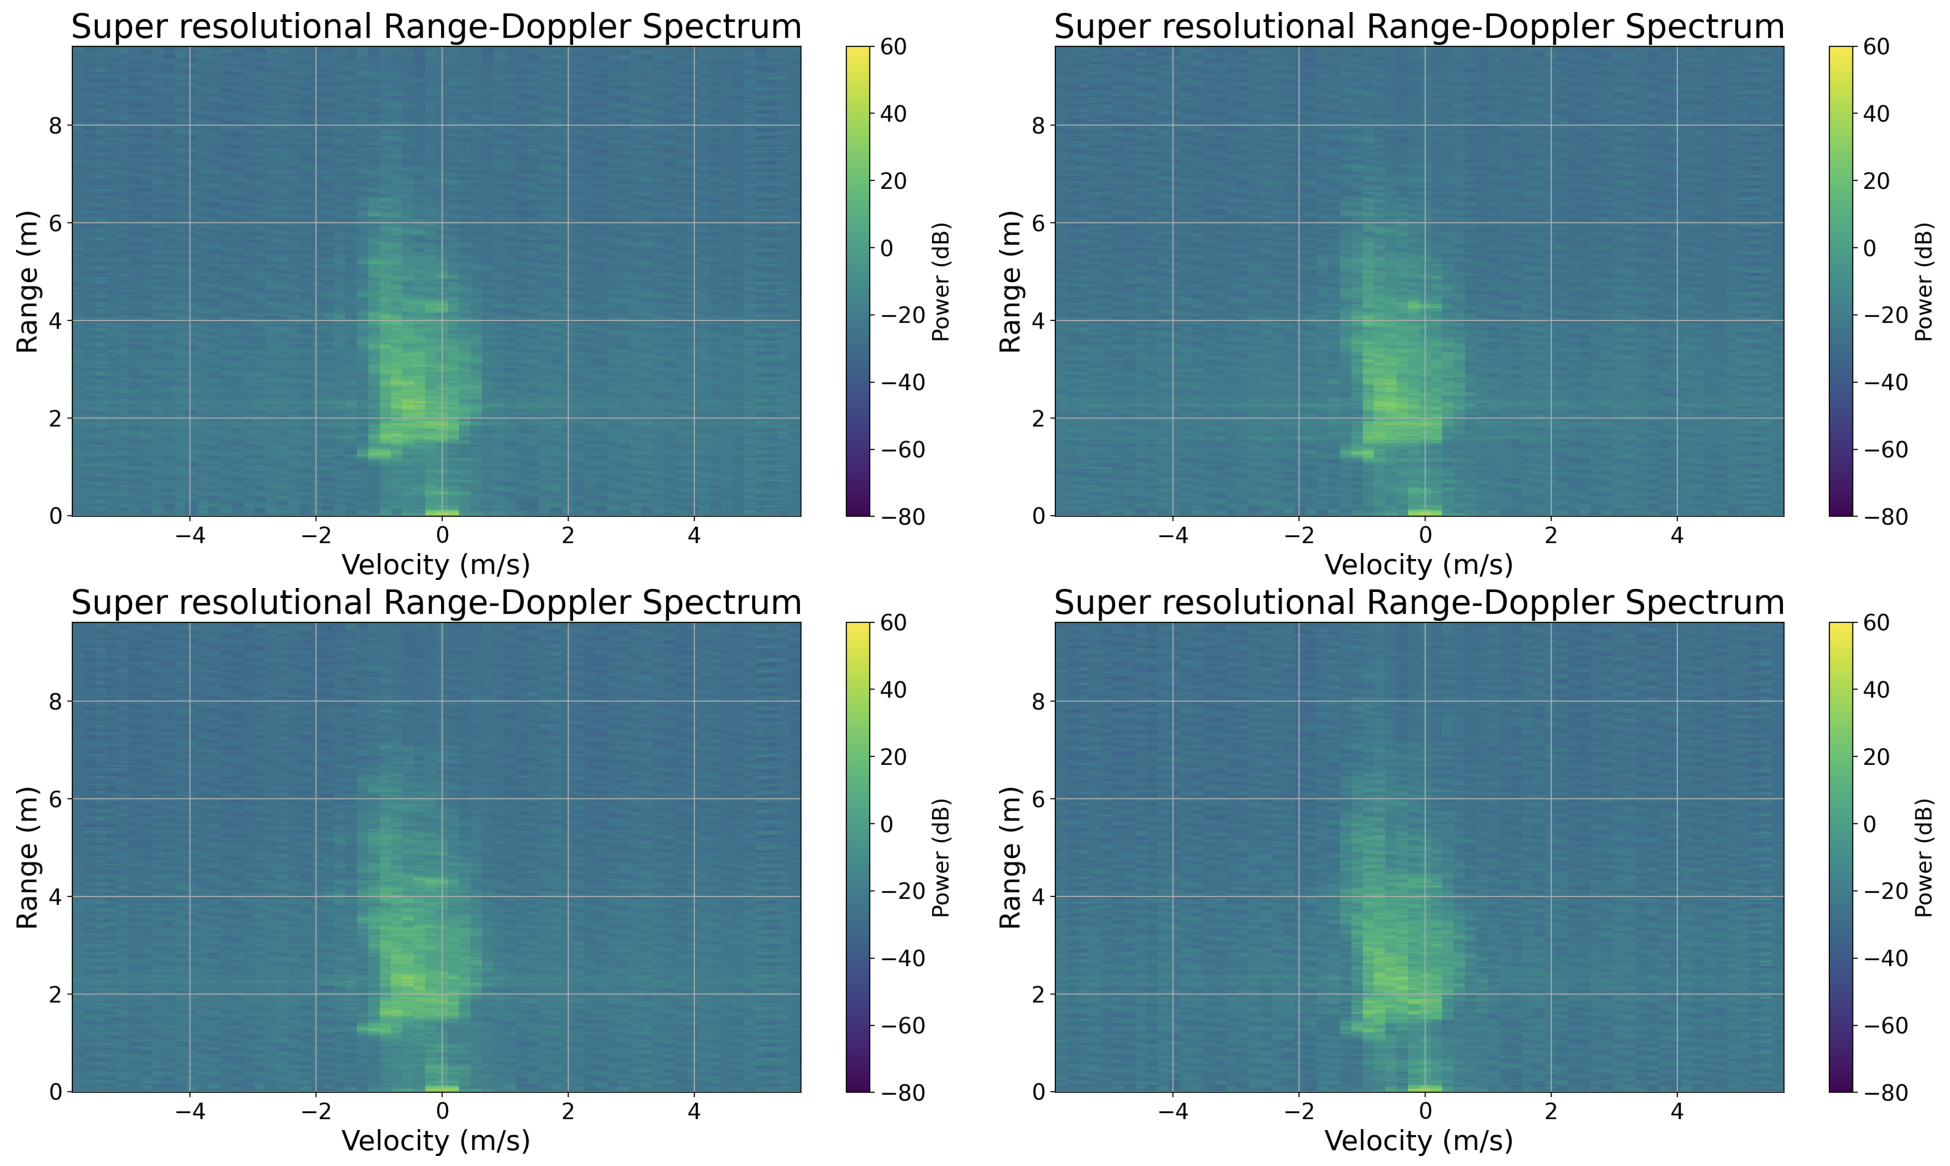
\includegraphics[scale=.45]{thesis/figures/evaluation_vgg.png}
    \caption{Super-resolution range-Doppler maps of different combinations of the VGG layers in the training loss combination, in the first row from left to right as b1c2+b2c2+b3c4 and b1c2+b2c2+b3c4+b4c4, in the second row as b1c2+b2c2+b3c4+b4c4+b5c4 and b2c2+b3c4+b4c4.}
    \label{Super-resolution images of different VGG layers}
\end{figure}


\section{Number of frames} \label{FOL comparison}
Since the range-Doppler map is always collected dynamically, that is, the continuous frames will have some relationship and the model could get more motion information. In this thesis, everything discussed previously is based on the setting that the number of frames in the inputs is 4. In this section, the effects of different numbers of frames values on the model will be evaluated. Table \ref{Evaluation losses of FOL comparison} and Figure \ref{Super-resolution images of different FOL values} illustrate the difference between the two cases.

From the evaluation losses from different cases, when the number of frames is chosen as 4, it can achieve a better result. Therefore, the continuous motion information is useful for the model and it verifies the previous assumption as well.

\begin{table}[!htp]
    \centering
    \caption{Evaluation losses of different numbers of frames values.}
    \label{Evaluation losses of FOL comparison}
    \begin{tabular}{l|c|c|c|c|c}
        \hline
        \#Frames comparison & MSE & SDR & LSD & WMSE & Perceptual \\
        \hline
        \multicolumn{6}{c}{\textbf{\#Frames = 1}}\\
        \hline
        DP & \textbf{1.379} & -5.239 & 0.381 & 0.191 & 12.778 \\
        \hline
        cGAN & 1.950 & -3.930 & 0.409 & 0.236 & 13.063 \\
        \hline
        \multicolumn{6}{c}{\textbf{\#Frames = 4}}\\
        \hline
        DP & 1.731 & \textbf{-5.375} & \textbf{0.380} & \textbf{0.179} & \textbf{12.320} \\
        \hline
        cGAN & \textbf{1.640} & \textbf{-5.690} & \textbf{0.374} & \textbf{0.169} & \textbf{11.881} \\
        \hline
    \end{tabular}
\end{table}

\begin{figure}[!htp]
    \centering
    \begin{subfigure}{0.95\textwidth}
        \centering
        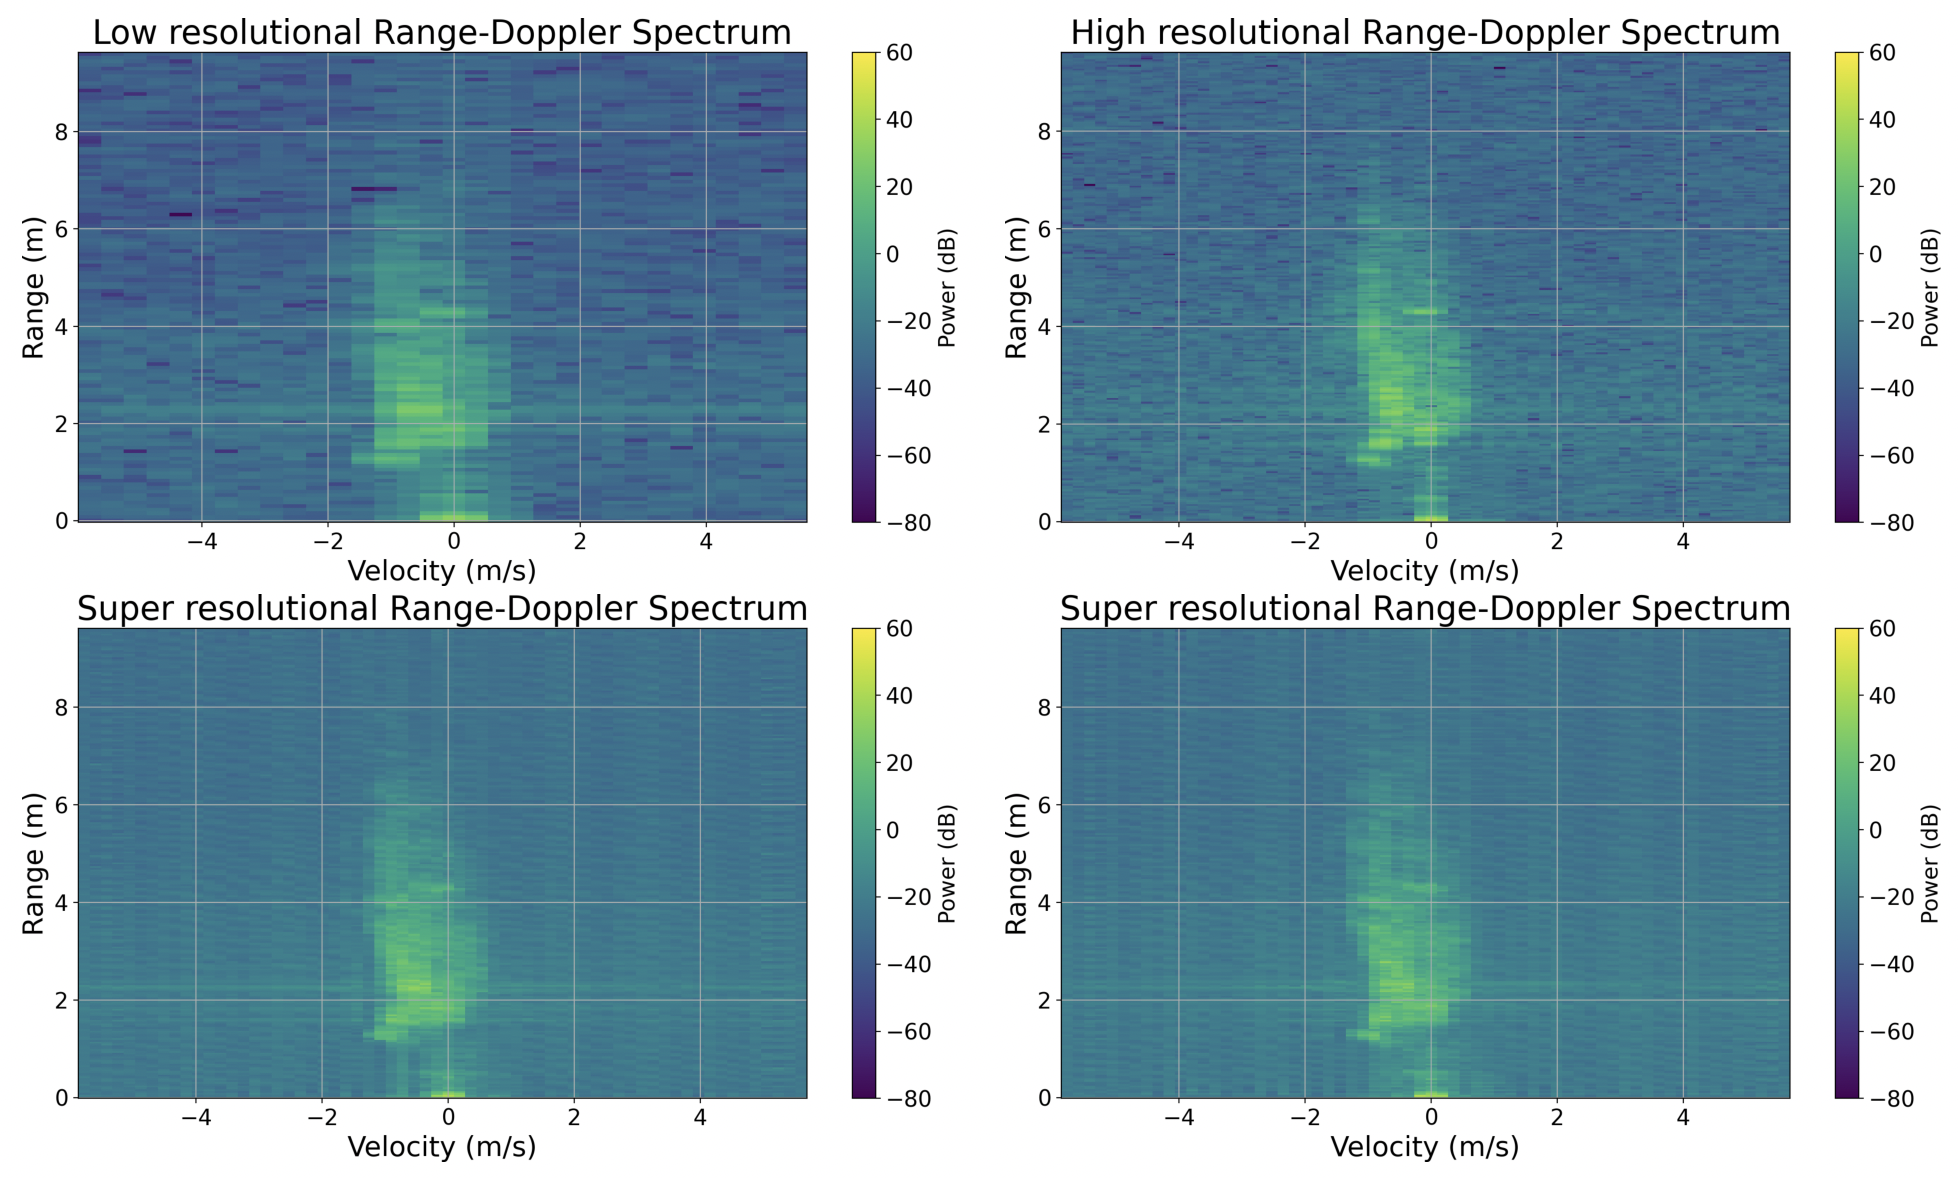
\includegraphics[width=\textwidth]{thesis/figures/evaluation_FOL1.png}
        \caption{Super-resolution range-Doppler maps with one frame as input, where in the second row the left from DP-TF Transformer model and the right from cGAN model.}
        \label{Super-resolution image while FOL value as 1}
    \end{subfigure}
    \vspace{0.3cm}
    \begin{subfigure}{0.95\textwidth}
        \centering
        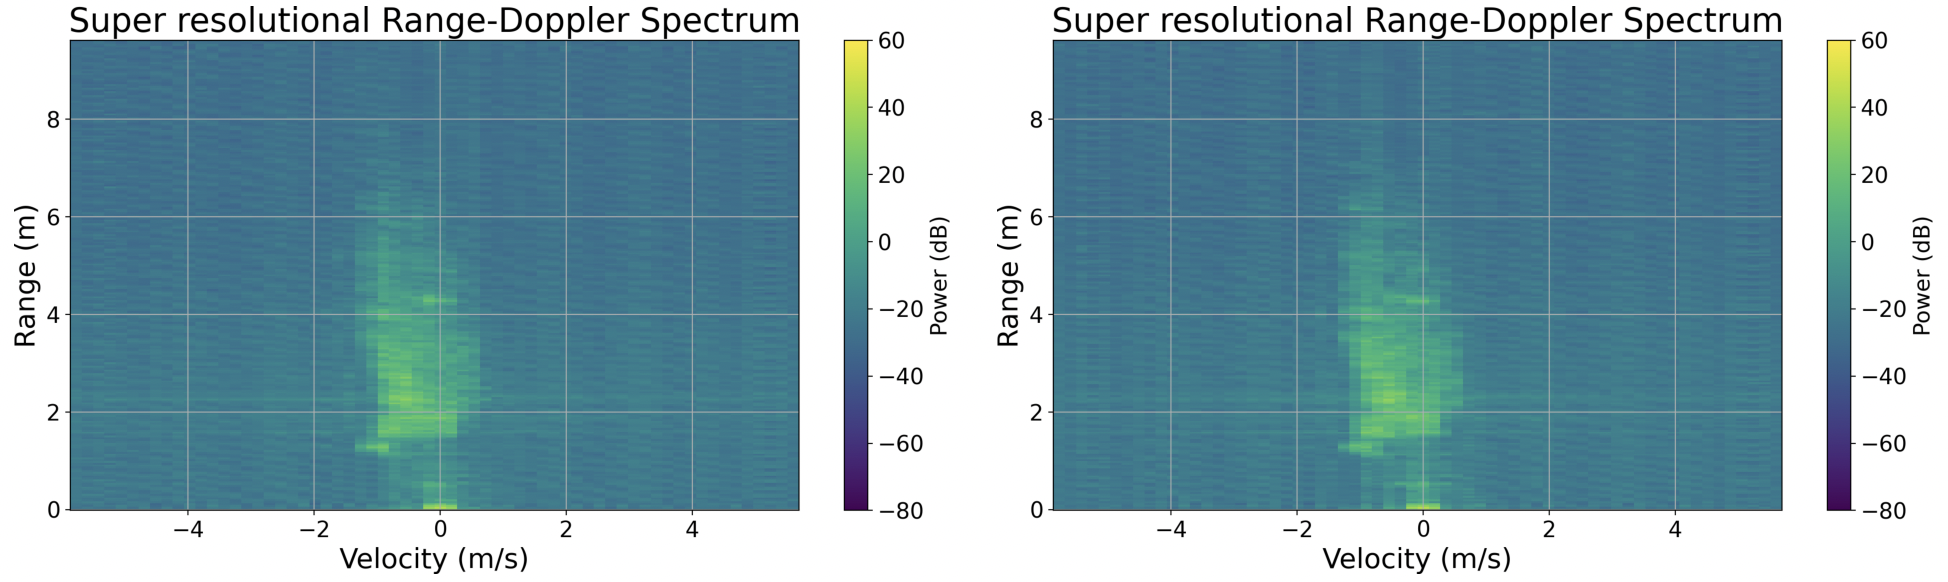
\includegraphics[width=\textwidth]{thesis/figures/evaluation_FOL4_under.png}
        \caption{Super-resolution range-Doppler maps with four frames as input, where the left from DP-TF Transformer model and the right from cGAN model.}
        \label{Super-resolution image while FOL value as 4}
    \end{subfigure}
    \caption{Super-resolution range-Doppler maps of different numbers of frames}
    \label{Super-resolution images of different FOL values}
\end{figure}

\section{Resampling rate} \label{Resampling rate comparison}
With the optimal processing methods and loss combination, the case that the 4$\times$ downsampled low-resolution range-Doppler map is evaluated with both \gls{dp}-\gls{tf} Transformer model and \gls{cgan} model in this section. Table \ref{Evaluation losses while the resampling rate as 4} and Figure \ref{Super-resolution images while the resampling rate as 4} show the results. However, the evaluation losses as well as the super-resolution range-Doppler maps look not as good as the case of 2$\times$ downsampled low-resolution range-Doppler map. The reason is that too much information is lost, only the shape of the part with high signal power can be seen.

\begin{table}[!htp]
    \centering
    \caption{Evaluation losses while the resampling rate as 4.}
    \label{Evaluation losses while the resampling rate as 4}
    \begin{tabular}{l|c|c|c|c|c}
        \hline
        Resampling rate & MSE & SDR & LSD & WMSE & Perceptual \\
        \hline
        DP & 2.208 & 5.811 & 0.620 & 0.491 & 22.347 \\
        \hline
        cGAN & 2.307 & 5.166 & 0.600 & 0.429 & 22.162 \\
        \hline
    \end{tabular}
\end{table}

\begin{figure}[!htp]
    \centering
    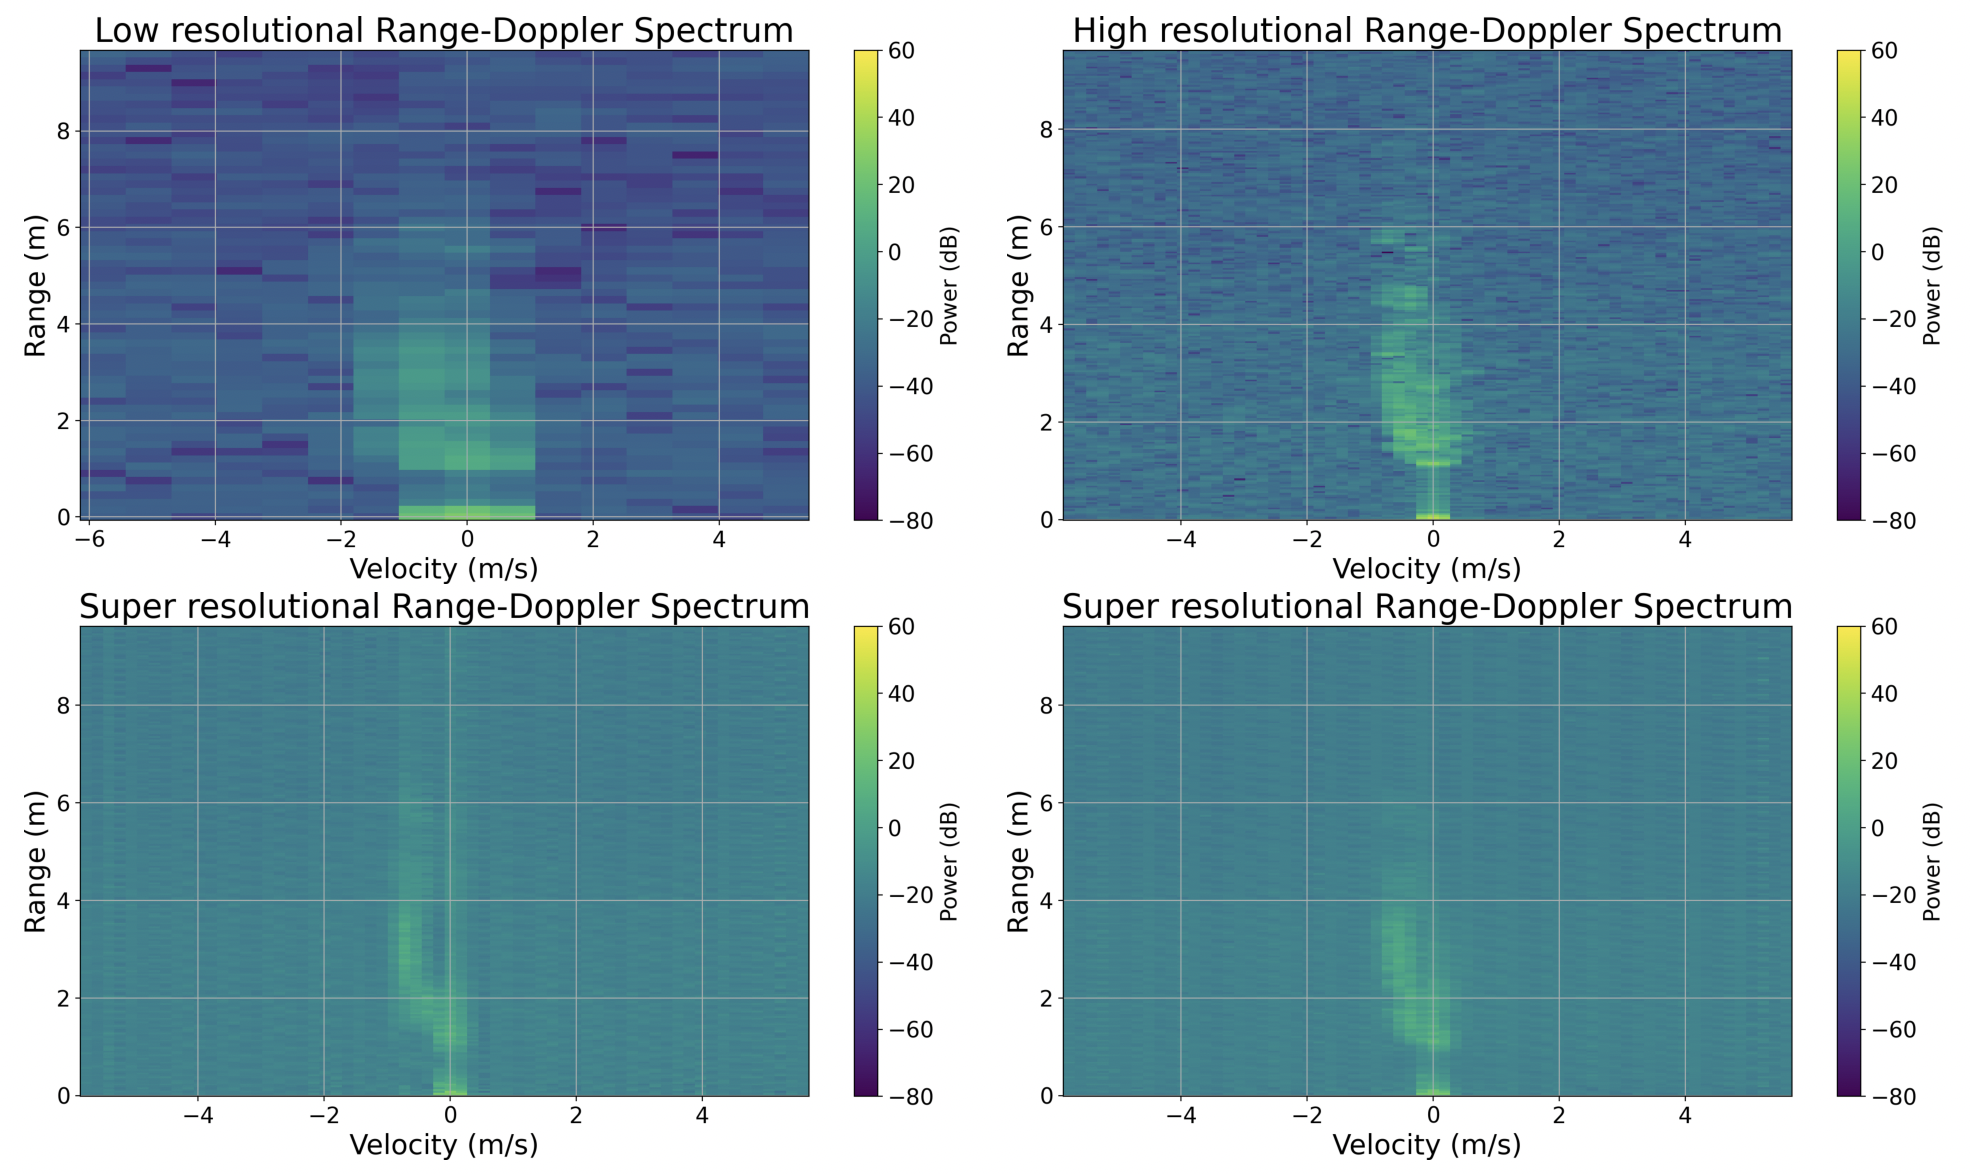
\includegraphics[scale=.45]{thesis/figures/evaluation_resampling4.png}
    \caption{Super-resolution range-Doppler maps while the resampling rate as 4, where in the second row the left from DP-TF Transformer model and the right from cGAN model.}
    \label{Super-resolution images while the resampling rate as 4}
\end{figure}

\section{Distributed training speed} \label{Distributed training evaluation}
To speed up the training process, the distributed training is used in the pipeline. The speed comparison is illustrated in Figure \ref{Evaluation of the speed by the distributed training}, which is recorded as the distributed training was successfully implemented, where \gls{dp}-\gls{tf} Transformer model is used in a large scale. The time taken in each epoch decreases from roughly 1800 seconds to under 400 seconds, that is, it uses multiple \gls{gpu}s successfully.


\begin{figure}[!htp]
    \centering
    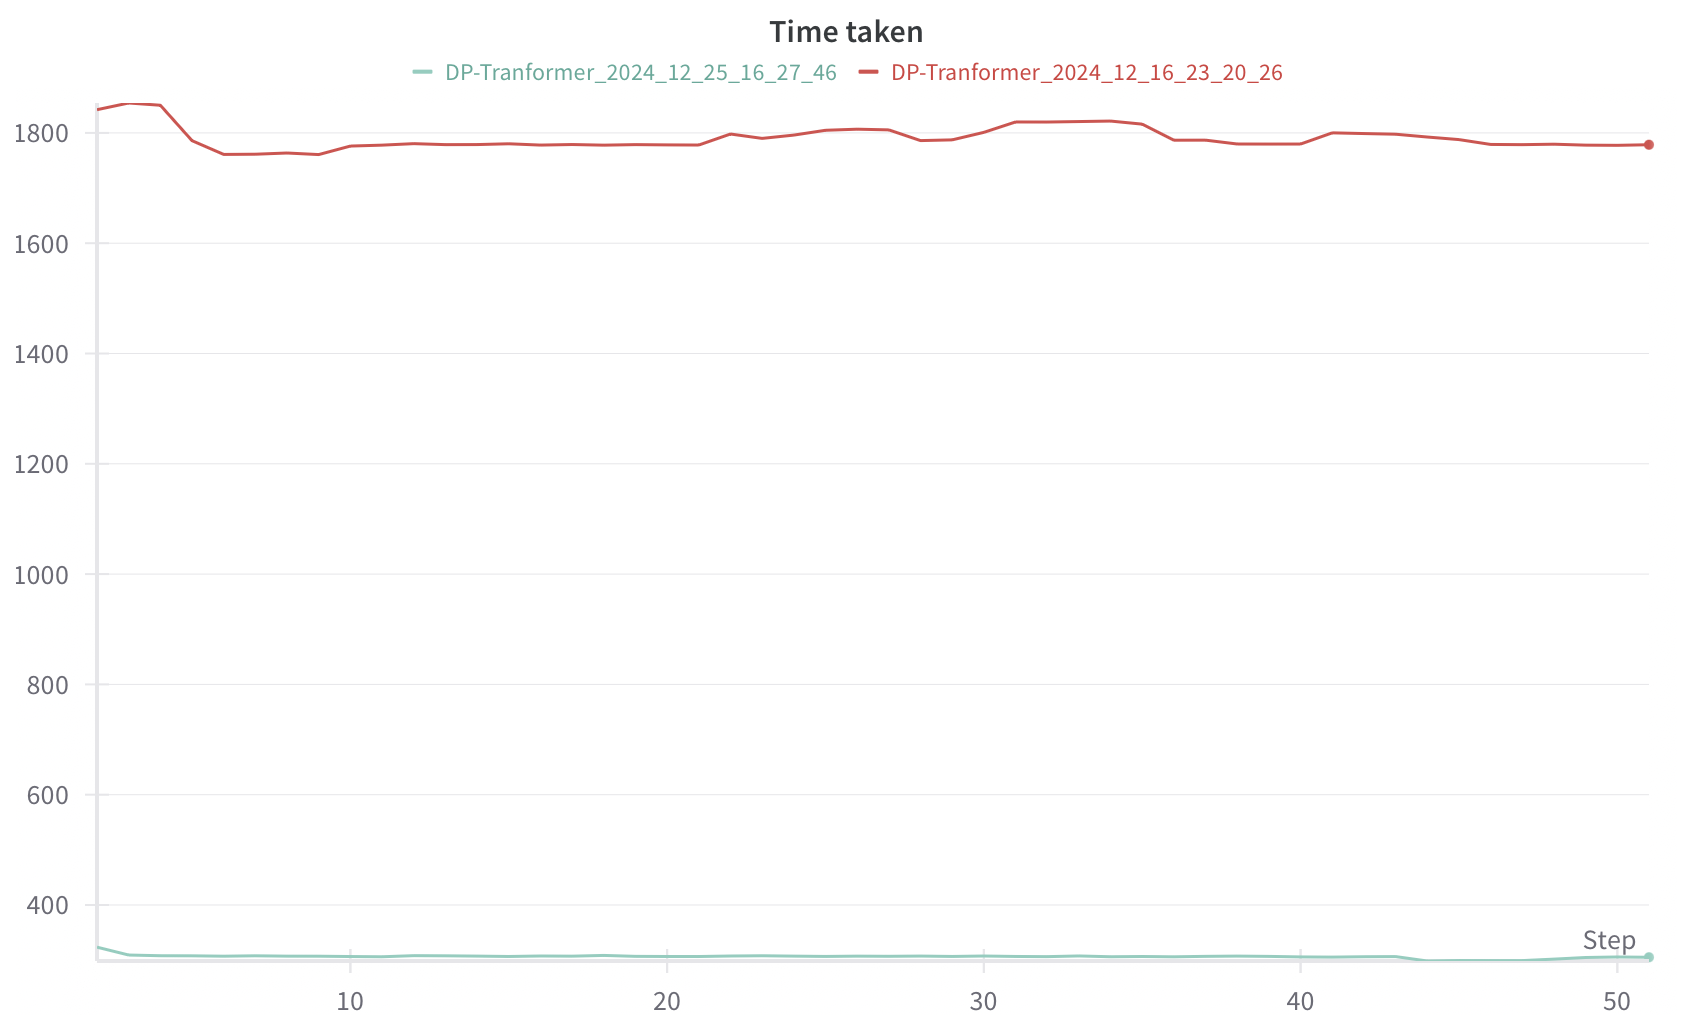
\includegraphics[scale=.45]{thesis/figures/evaluation_distributed_training.png}
    \caption{Evaluation of the speed by the distributed training, where the red line represents the pipeline without distributed training while cyan line with.}
    \label{Evaluation of the speed by the distributed training}
\end{figure}


\section{Hyperparameters tuning} \label{hyperparameters tuning evaluation}
The hyperparameters of the model and training process have an impact on the result, such as the number of blocks, the number of filters, etc. Therefore, in this section, the sweep function in \gls{wandb} is used to combine and evaluate some hyperparameters to find a better combination that minimizes the loss. Figure \ref{Hyperparameters tuning by WandB} shows the sweep process of \gls{wandb}. With optimal combination of the hyperparameters, the evaluation losses and the visual effect of the super-resolution range-Doppler maps have improved as shown in Table \ref{Evaluation losses after hyperparameters tuning} and Figure \ref{Super-resolution images after the hyperparameters tuning}.

\begin{figure}[!htp]
    \centering
    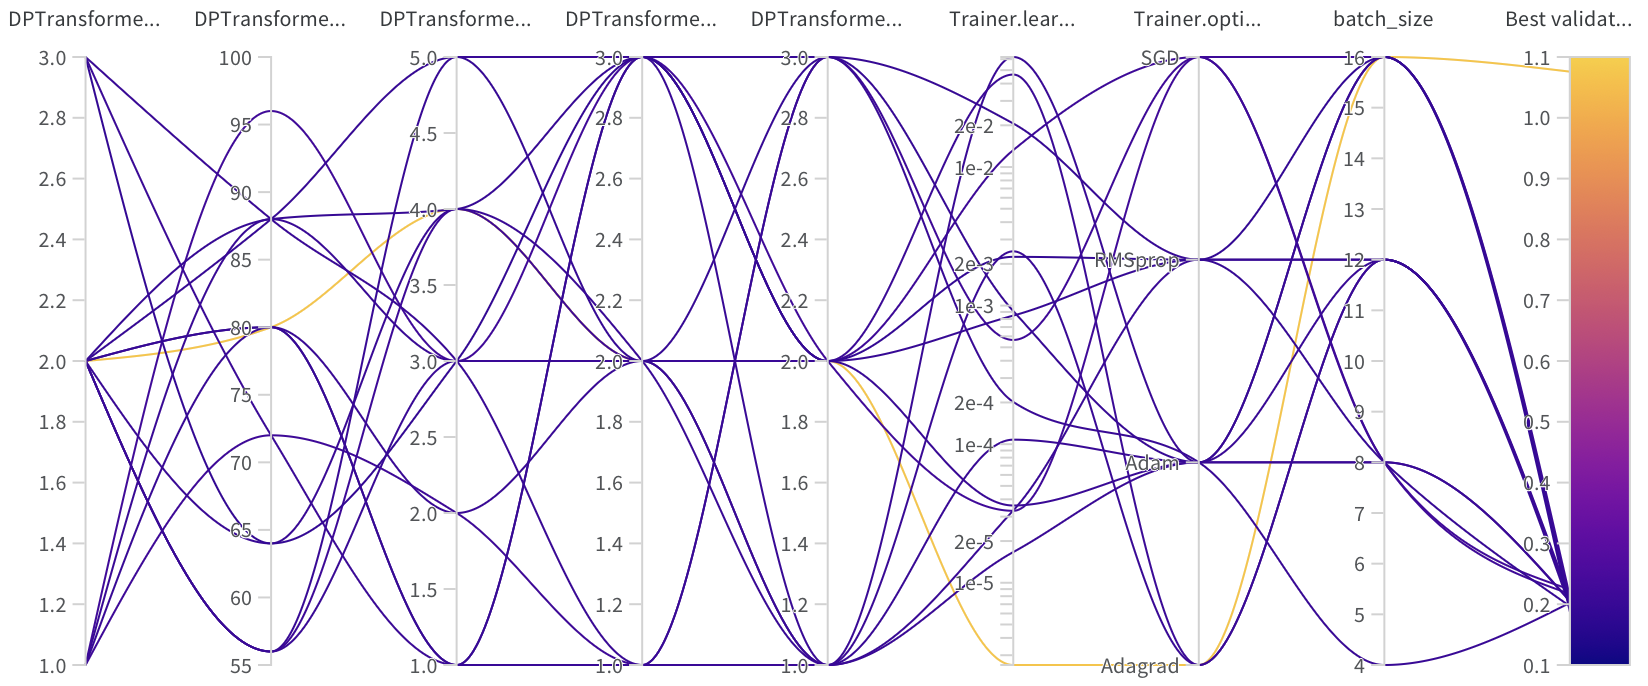
\includegraphics[scale=.54]{thesis/figures/evaluation_hyperparameters_tuning.png}
    \caption{Hyperparameter tuning by WandB}
    \label{Hyperparameters tuning by WandB}
\end{figure}

\begin{table}[!htp]
    \centering
    \caption{Evaluation losses after hyperparameters tuning}
    \label{Evaluation losses after hyperparameters tuning}
    \begin{tabular}{l|c|c|c|c|c}
        \hline
        Hyperparameters tuning & MSE & SDR & LSD & WMSE & Perceptual \\
        \hline
        DP & 1.225 & -5.625 & 0.373 & 0.146 & 11.753 \\
        \hline
        cGAN & 1.223 & -5.187 & 0.382 & 0.157 & 10.915 \\
        \hline
    \end{tabular}
\end{table}

\begin{figure}[!htp]
    \centering
    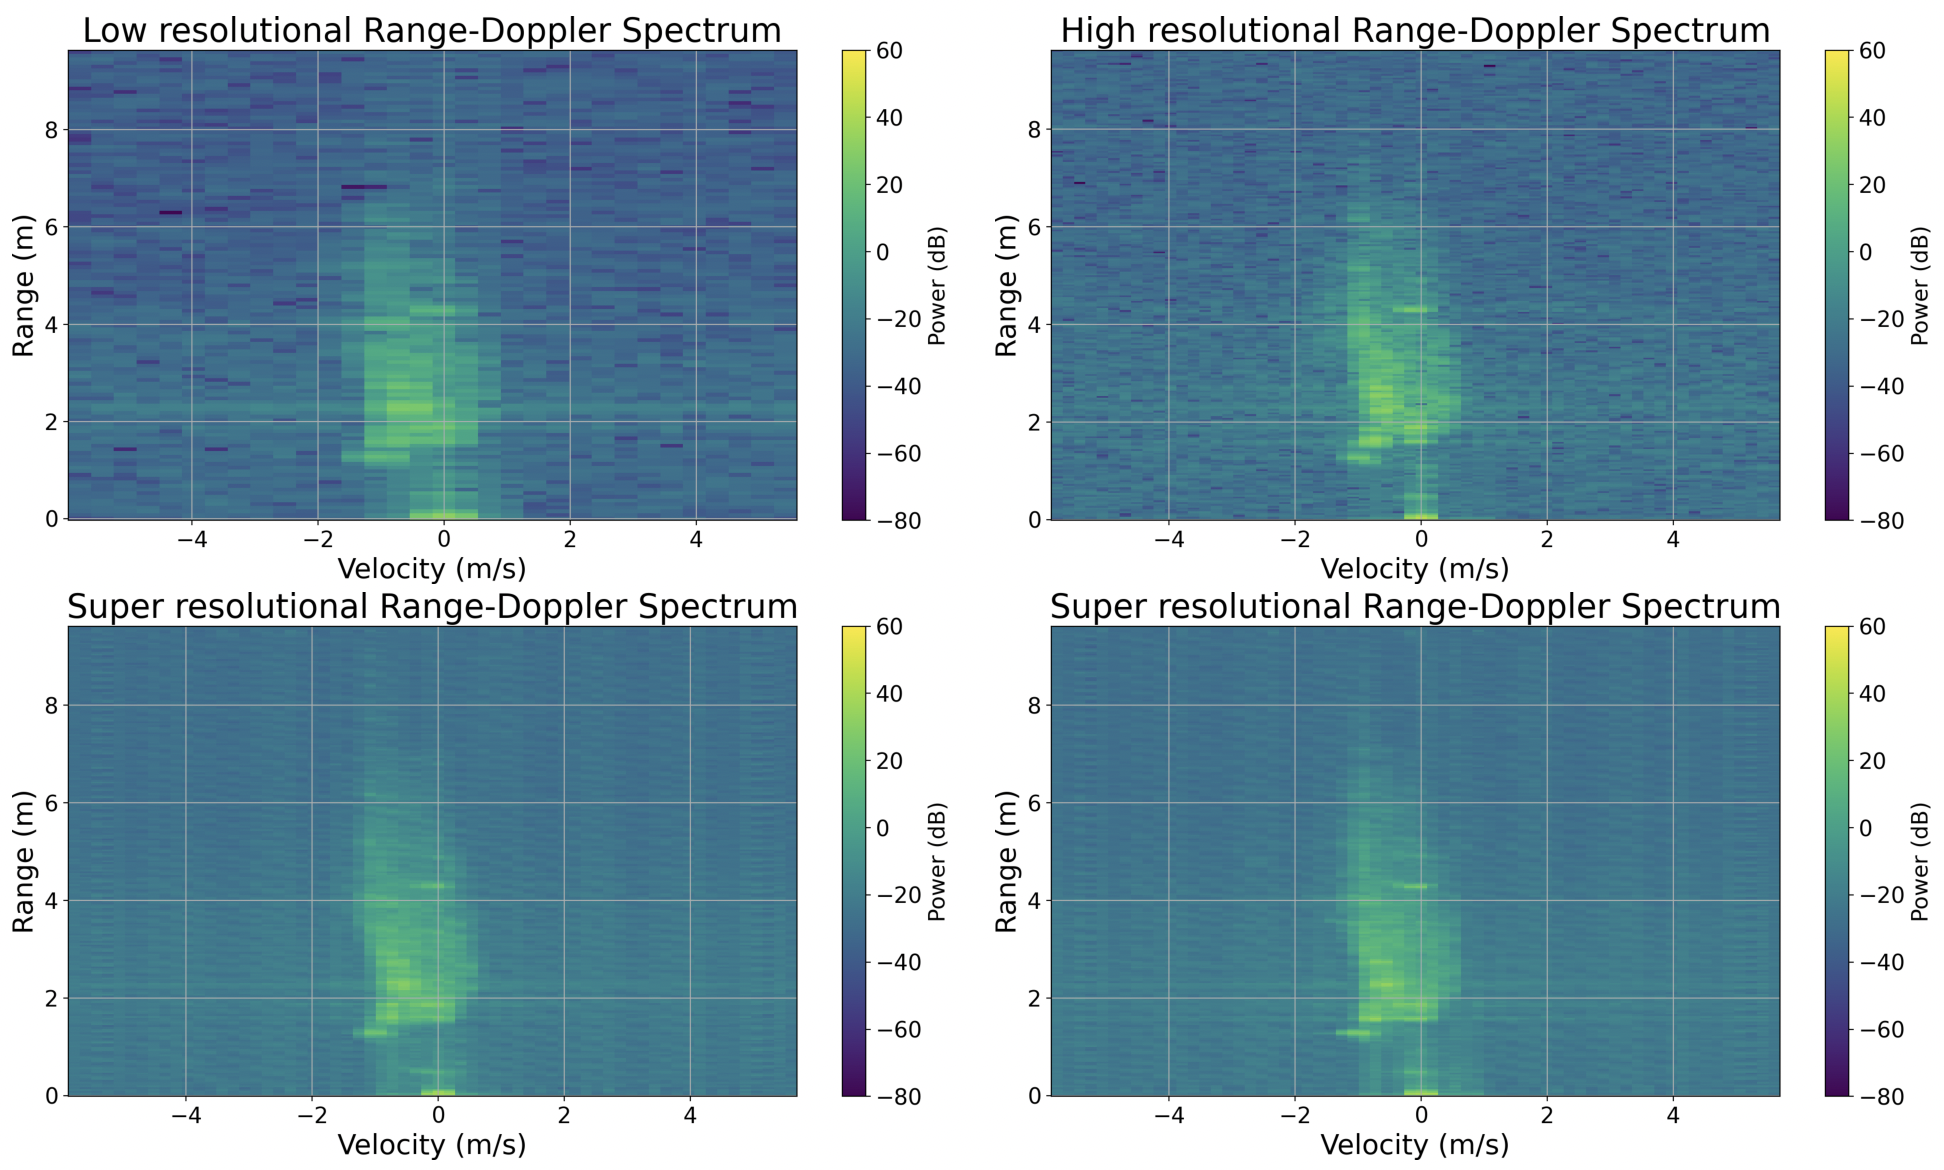
\includegraphics[scale=.4]{thesis/figures/evaluation_tune.png}
    \caption{Super-resolution range-Doppler maps after the hyperparameters tuning, in the second row left on trained by DP-TF Transformer model while right one trained by cGAN model.}
    \label{Super-resolution images after the hyperparameters tuning}
\end{figure}


\section{Final result} \label{final result evaluation}
Keeping the same tuned hyperparameters as evaluated in section \ref{hyperparameters tuning evaluation}, after running more epochs with the large model as well as the whole dataset, the evaluation losses and super-resolution range-Doppler maps are further improved as shown in Table \ref{Evaluation losses with large models and whole dataset} and Figure \ref{Super-resolution images trained by large models and whole dataset}.
% The reason about the perceptual loss from \gls{cgan} model no longer smaller than \gls{dp}-\gls{tf} Transformer model would be that the scale of the discriminator is not large enough, when the large generator and the whole dataset are used, the generator improves a lot while the limit of the discriminator is reached.

\begin{table}[!htp]
    \centering
    \caption{Evaluation losses with large models and whole dataset, where the number of parameters of the DP-TF Transformer model and the generator is 329,410 while that of the discriminator is still 766,187.}
    \label{Evaluation losses with large models and whole dataset}
    \begin{tabular}{l|c|c|c|c|c}
        \hline
        Final result & MSE & SDR & LSD & WMSE & Perceptual \\
        \hline
        DP & 0.968 & -6.008 & 0.363 & 0.123 & 9.079 \\
        \hline
        cGAN & 0.803 & -5.619 & 0.371 & 0.120 & 8.740 \\
        \hline
    \end{tabular}
\end{table}

\begin{figure}[!htp]
    \centering
    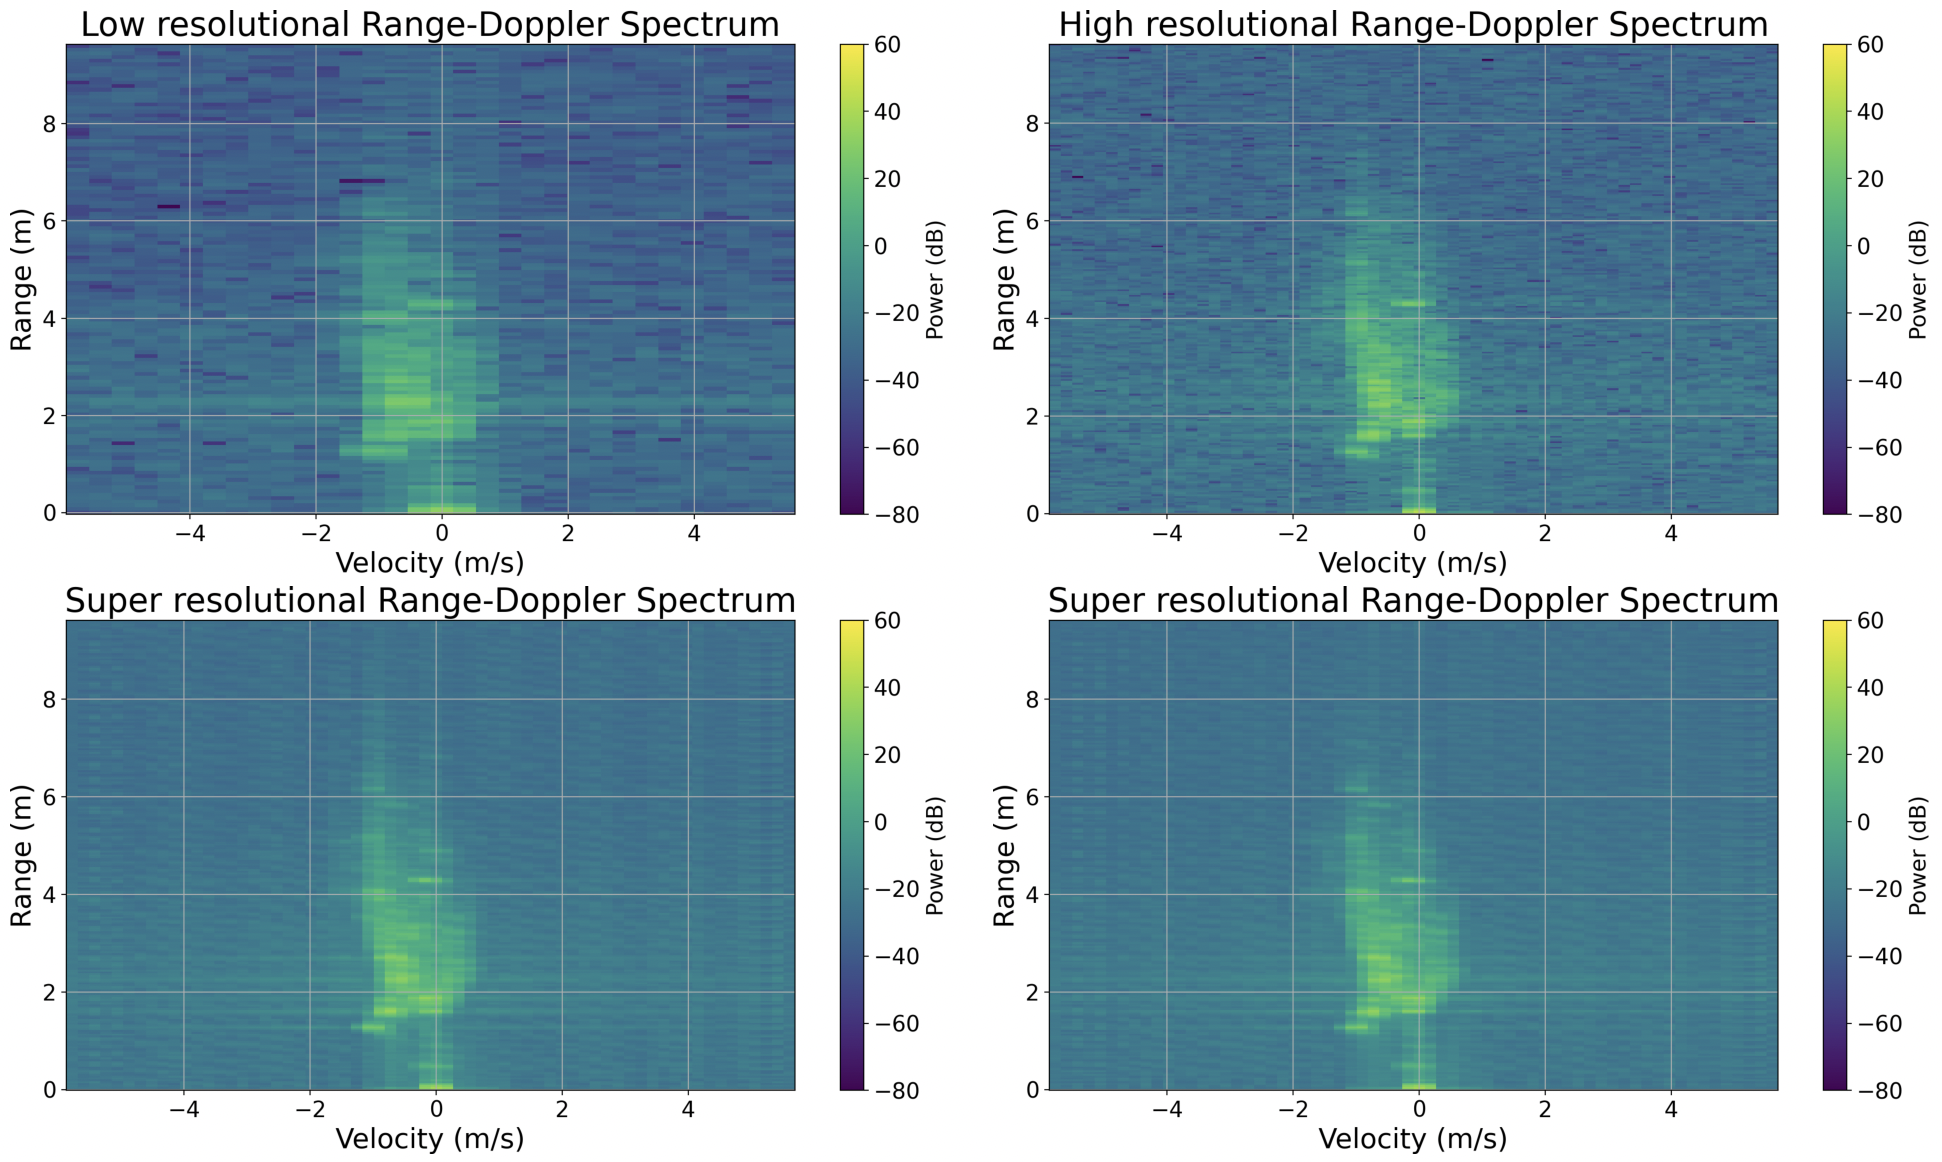
\includegraphics[scale=.4]{thesis/figures/evaluation_large_new.png}
    \caption{Super-resolution range-Doppler maps trained by large models and whole dataset, in the second row left one trained by DP-TF Transformer model while right one trained by cGAN model.}
    \label{Super-resolution images trained by large models and whole dataset}
\end{figure}